%----- Author : Kang Yen -----%
%----- Version: 1.0        -----%
%----- Date   : 2019.06    -----%

\documentclass[12pt]{ksthesis}
\usepackage[cmex10]{amsmath}
\usepackage{amsthm}
\usepackage{latexsym}
\usepackage{./class/psfig}
\usepackage{./class/fancyheadings}
\usepackage{./class/citesort}
\usepackage{graphicx}
\usepackage{subfigure}
\usepackage{amssymb}
\usepackage{algorithm}
\usepackage{algorithmic}
\usepackage{multirow}
\usepackage{cite}
\usepackage{caption}

\newtheorem{thm}{Theorem}
\newtheorem{lemma}{Lemma}
\newtheorem{defi}{Definition}
\newtheorem{proposition}{Proposition}
\newtheorem{cor}{Corollary}

\paperwidth=21cm \paperheight=29.7cm

\doublespace

\title{National Cheng Kung University
     \\Institute of Computer and Communication Engineering
     \\Master Thesis}
\author{}

\phdthesis

\Thesisspace

\begin{document}

\begin{preliminary}
%---------- Preliminary ----------%
\setcounter{page}{2} \large


\begin{abstract}
%------------------------- Abstract -------------------------%
\begin{center}

{\Large A Mobile App with Real-Time Vehicle Dispatching in a Self-Driving Delivery System\vspace{0.4cm}}

\end{center}

\begin{center}

{\large Jyun-Ting Po\vspace{0.2cm} \\ Institute of Computer and
Communication Engineering \vspace{0.2cm}\\ National Cheng Kung
University \\ }

\end{center}

\Thesisspace {\large 
With the development of self-driving technology in the recent years, a lot of related industries and the applications gradually popped up. Among the applications, the freight transport and the sale of driverless trucks became a crucial research topic. However, due to the complexity of the road network and the constraint of traffic regulation, self-driving technology development companies have the difficulties with the complete system integration. Therefore, the thesis proposed a mobile application in a self-driving delivery emulation system. By using the dispatch mechanism, the application simulates the real user scenario of the parcel delivery service. As a result, the application can be view as a test platform before the application is officially launched. In the system, self-driving technology development companies can implement their own path planning algorithm and evaluate the effectiveness of the delivery process. Moreover, the user can interact with the system by the parcel delivery order from the mobile device, which leads to a more real delivery situation.

The thesis simulated a real-time parcel delivery service in urban-scale areas, built a database, and establish the socket interface between the simulator and the mobile application. Besides, the service contains the whole delivery process, which includes the pick-up of the cargo and the unloading task of parcels. Finally, the simulation result showed the compatibility for the ordinary delivery applications and offered the flexibility to adjust different logistics planning algorithms.  
}

\emph{\textbf{Keywords}}---self-driving, real-time, mobile application, parcel delivery service, traffic simulators

\end{abstract}

\begin{acknowledgements}
%------------------------- Acknowledgement -------------------------%
\Thesisspace {\large }

\end{acknowledgements}

\tableofcontents \listoffigures\clearpage

\end{preliminary}
%---------- Preliminary ----------%
\begin{thesis}\large {
%------------------------- Introduction -------------------------%
\chapter{Introduction} \label{Chap:Introduction}

Nowadays the world’s online marketplaces are growing rapidly, it is because the online shopping has the advantages of lower price and rapid delivery service. The total ecommerce sales increased last year by 20\% to \$1.66 trillion according to Internet Retailer’s released 2019 Online Marketplaces Report. [1] However, as the rapid development of e-commerce such as Amazon, Alibaba and eBay, it brings the novel problems and concerns. Compared to the tradition retailing, online shopping encounters lots of challenges. For consumers’ part, they must wait for the goods to arrive home instead of getting them immediately. Hence, the delivery time is a crucial factor for the consumer experience, and the parcel distribution becomes more and more important. 

%%%%%%%%%%%%%%%%%%%%%%%%%%%%%%%%%%%%


%%%%%%%%%%%%%%%%%%%%%%%%%%%%%%%%%%%%

\begin{figure*}
\footnotesize
\begin{minipage}[t]{0.48\linewidth}
    \centering
    \includegraphics*[width=\linewidth]{./figures/F1-a.PNG}
    (a)
\end{minipage}
\begin{minipage}[t]{0.48\linewidth}
    \centering
    \includegraphics*[width=\linewidth]{./figures/F1-b.PNG}
    (b)
\end{minipage}
\normalsize
\caption{First two big United Parcel Service of America Inc.'s revenue.}
\label{fig:UnitedParcelService}
\end{figure*} 

Figure 1.1 shows the revenue of two freight delivery companies, which have the highest market shares of couriers and local delivery service in the United States [2]. The trend chart represent that the demands of the express delivery service are growing year by year. In the domain of the express delivery, the same-day delivery is a significant service. It aims to shorten delivery time as much as possible to improve the customer satisfaction. In the future, performing parcel delivery by self-driving vehicles is a promising way to improve the efficient of route arrangement and reduce labor cost, thereby it can make it easier to achieve the same day delivery.

A self-driving vehicle, also known as a robotic vehicle, autonomous vehicle, or driverless vehicle, is a vehicle which is able to sense the surrounding environment by sensors and drive on the road without a human driver. In Intelligent Transport System (ITS), the self-driving vehicle usually has one of many different communication technologies to communicate with other vehicles and the control center in the same system. With the self-driving technology becoming mature gradually, more and more companies invested in the development of self-driving vehicles, such as Google, Tesla, Waymo, Baidu, and so on. 

However, in many country, it is difficult and challenging to test the vehicles on public roads due to the complex road environment or policy restrictions. Therefore, this thesis proposes a self-driving delivery system which combines the mobile applications with the traffic simulation software. The system aims to simulate the process of the same-day delivery in urban areas. By this system, the self-driving technology development companies can test and adjust their path planning algorithm, vehicle deployments and the different system function before the self-driving product is official online. The mobile application is exploited to simulate the real usage situation and improve the user experience. In contrast with traditional home delivery service [3] which does not allow the parcel receiver to select the expected delivery time, the proposed application provides the real-time vehicle dispatching. This means the user, including sender and receiver can select the arrival time of trucks at any time so that the failure rate of parcel delivery can be declined. 

The simulation system contains real-world road information, such as the longitude and latitude of the vehicle, the cycle time of traffic light, the different road types, and so on. The self-driving development companies can accomplish their expected function by these data. Besides, this thesis designs an interface and the data format of the data transmission. Thus, the mobile application can be easily integrated into the actual autonomous vehicles. By these advantages of this system, the self-driving vehicles can move seamlessly from the simulation to the real world. 

The remainder of this thesis is organized as follows. Related work is discussed in Chapter 2. The system design, system functions and the usage scenarios are described in Chapter 3. Chapter 4 illustrated the implementation of this system and the simulation environment. Finally, Chapter 5 concludes the thesis and discusses the future work.



  


\chapter{Related Work} \label{Chap:Related}
%------------------------- Related Works -------------------------%

According to Data Booklet of United Nations [4], the number of cities with at least 1 million citizens is 548 in 2018, and it will grow to 706 in 2030. As a result, city logistics are getting more attention. The goal of City logistic issues is to find efficient and effective ways to transport goods in urban areas. There are some studies discussing the current opportunities and challenges of city logistics. [5][6]
 
Last mile is the delivery process that transport goods to the final destination within the city. Habault et al. presented a delivery management system architecture. [7] The system uses the data generated from the machine-learning mechanism to reduce the delivery travel time. Ewedairo et al. used a scenario thinking approach to identify the potential planning and transport systems attributes that would obstruct the last mile delivery. [8] It mentioned that the modes of transportation have great impact on delivery costs. Hochstenbach et al. introduced the design of an unmanned aerial vehicle (UAV) for autonomous parcel delivery. [9] Niels et al. presented a project in Munich, Germany, where the last mile package delivery is carried out by cargo bikes and eBikes. [10] GUO et al. presented a framework which exploits the underutilized capacity of crowdsourced public transportation systems (CPTS) such as the bus or the subway to perform the same-day parcel delivery. [11]

Utilizing the self-driving vehicles to perform the parcel delivery is a novel and attractive research direction. Buchegger et al. proposed an autonomous transport vehicle which is capable of navigating in large-scale urban environments. [12] The vehicle in this study is based on a commercially available electric vehicle, and it had been adapted for autonomous operation. A new delivery framework for same-day delivery was proposed in [13]. The goods are delivered to a nearby pickup station so that it can alleviate many of the shortcomings that autonomous vehicles have. Kocsis et al. presented a service in smart cities for delivering grocery using autonomous vehicles in urban areas. [14] The autonomous vehicles in this study was developed using an electric golf cart by the same authors.


Seth et al. presented a system named Similitude comprised of the SimMobility traffic simulator coupled with Android emulators and an optional network simulator (ns-3). [15] Compared to our system, Similitude focuses on the general transportation and it does not support the user interaction interface.




\chapter{System Design}\label{Chap:System_design}


\section{System Overview}

\begin{figure}[H]
\centering
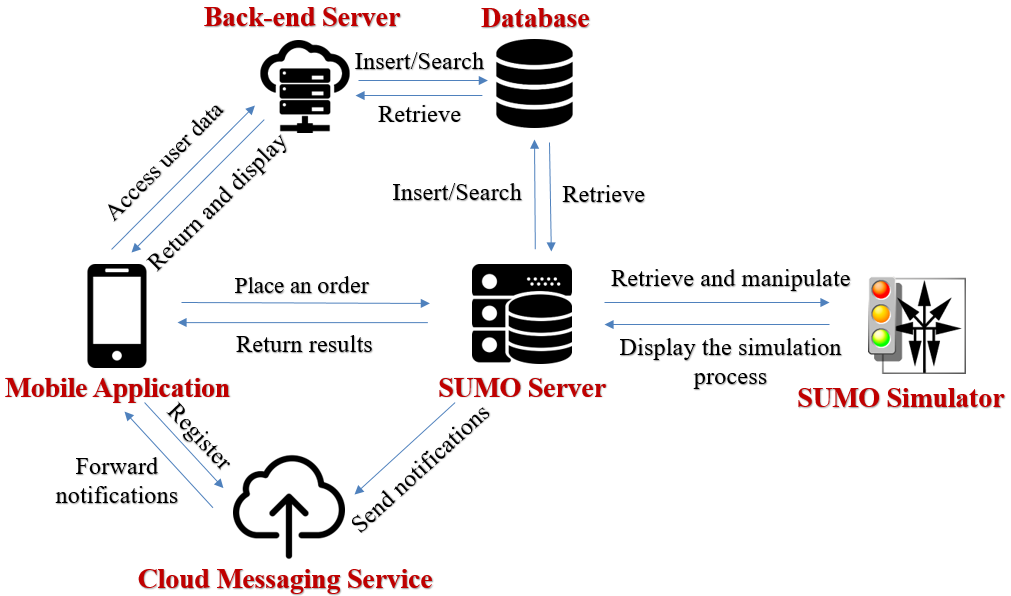
\includegraphics[width=1.0\textwidth]{./figures/F3-1_SystemOverview.PNG}
\caption{\large System overview.}
\vspace{0.5cm}
\label{Fig:system_Overview}
\end{figure}

This thesis designs a self-driving delivery simulation system, as illustrated in Figure 3.1, the system consists of five components, including the mobile application, the SUMO server, the SUMO simulator, the back-end server, and the database. 

In this system, the mobile application is a platform which can let the user place a delivery order for shipping cargos and track the user’s orders. After a user issues a delivery request on the mobile application, the request will be sent to SUMO server. The server will execute the dispatching mechanism to assign a truck which meets the conditions to receive the cargo, and the movement of the truck will be displayed on SUMO simulator by commands of SUMO server. 

Moreover, the information of orders will be uploaded to the database if the assignment is successful, and the user can check the order’s status on the mobile application by connecting to the back-end server. When the truck arrives at the address of shippers or receivers on the simulator, the SUMO server will send a message to the mobile device for notifying the user of this arriving event through a cloud messaging service. 

Besides, the server will also send a message to notify the receiver that the pickup time of the cargo can be selected already when the truck has arrived at the sender’s address. All the simulated process can be observed on the SUMO simulator. The features of each component will be described in detail in the following sections.

\section{Mobile Application}
In this system, the main object to develop the mobile application is to simulate the real user scenario. The features of the mobile application include registration and login of the user accounts, placing the delivery order, and tracking established orders. The function of each part is depicted as follows.

\subsection{Registration and Login}
When the mobile application is launched for the first time, a token will be generated. If a user sign up and sign in his/her account, the token will be uploaded to the database. The SUMO server can send a notification to the mobile device by this token while the truck arrives at the target. On the other hand, the user-related data like username will be stored in the device’s memory when the user sign in, and it can be used to generate the delivery order and track the user’s history orders. The process will be described in the next two sections.

\subsection{Placing a Delivery Order}
In order to simulate the real user scenario, the thesis implements a function that the user can place an delivery order. First, the user needs to fill out the order’s information which includes container size, receiver’s username, sender’s address, receiver’s address, and so on. 

Then, the address will be displayed by Google Map service so that the user can confirm the correction of localization. After that, the user can choose the arrival time of the truck, and send the delivery request to the SUMO server. The request contains user-related data and the details of the order, and the server will run the dispatching mechanism by the information and the road condition of the SUMO simulator. The order will be uploaded to the database if the request is accepted. Otherwise, the SUMO server will return a error message to the application to notify the user that there is no truck which can arrive the destination at the appointed time.

\subsection{Tracking Established Orders}
After the order is established successfully, the user can track the orders’ status by using the function of tracking orders. In this function, \textbf{the user is divided into two categories including a receiver and a sender}.

Besides, if the user is a receiver, he can choose the pickup time of the cargo after the truck arrives at the sender’s address.  
Moreover, the receiver only can select the pickup time after the cargo is load into the truck because the system must ensure the cargo is ready to be delivered. 
In addition, the system provides a function to examine the orders by inputting the order number instead of login. the function let the administrator can search all orders of users conveniently on the mobile device.

\section{SUMO Server and SUMO Simulator}
In this system, the SUMO server is response for receiving the user’s requests of delivery, executing the dispatching mechanisms, and updating the orders of users, and communicating with the SUMO simulator to get the data of road conditions and dispatch the truck to the destination on the simulator. This thesis deals with processing of received data and uploading the orders to the database.

\begin{figure}[H]
\centering
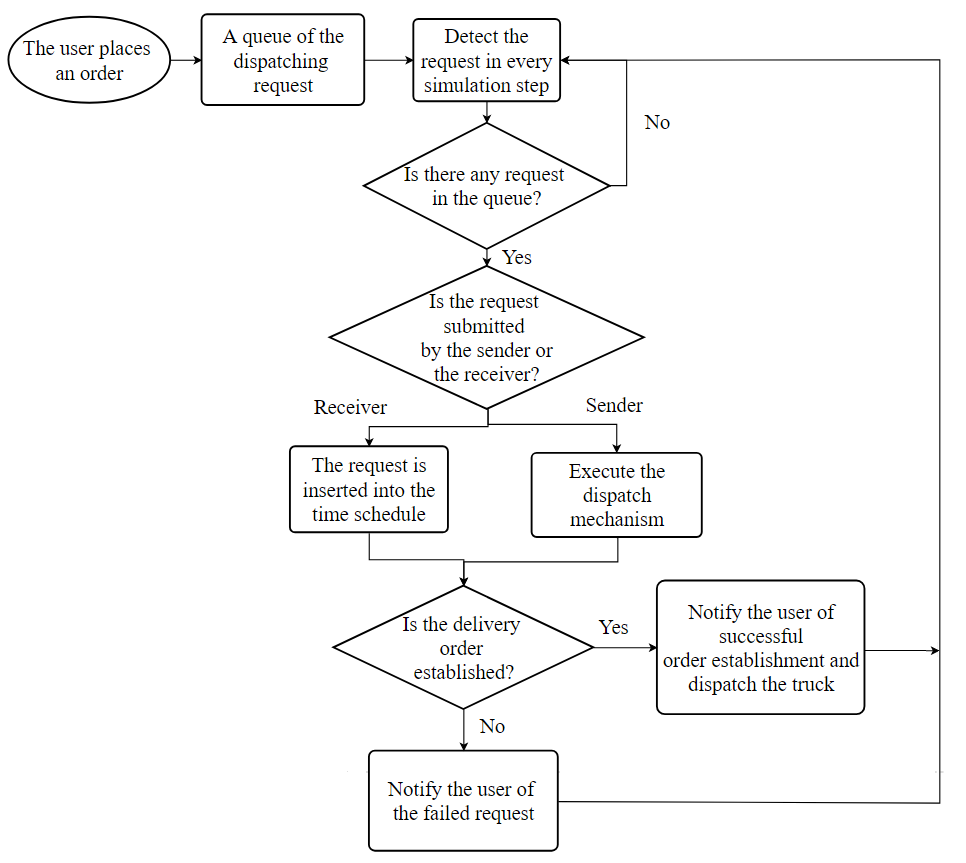
\includegraphics[width=1.0\textwidth]{./figures/F3-2_Flowchart.PNG}
\caption{\large Flow chart of the delivery process.}
\vspace{0.5cm}
\label{Fig:flow_chart}
\end{figure}




As illustrated in Figure 3.2, after the user places an order with the SUMO server, the order will be stored in a queue of the dispatching requests. The socket program can detect the request whether it is sent by a sender or a receiver according to the data, and the server will store extra information like the truck number and the container number if the request is sent by a receiver. 
It is because that the server needs to know which trucks to be dispatched. The server will check the queue continuously, and do the dispatching mechanism if there are any requests in the queue. If the dispatching is successful, the server would insert or update the order to the database with the database API and send a message to the mobile application through the socket. Otherwise, the server will notify the user that this arrival-time is unavailable with error message. 

Moreover, the SUMO server will change the dispatching schedule table on the basis of the above result, and it will execute the corresponding commands to the SUMO simulator so as to change the selected the truck’s route.
After the delivery tasks are assigned to the trucks, they will drive along the designated routes, and the system administrator can observe the trip and the parking place of each truck in the simulator. When a truck arrives at the destination, the SUMO server will send a notification to the mobile device through the cloud messaging service. 
When the truck arrives to the destination and then five minutes passes, the server will simulate the uploading and unloading task, and the server will also notify the receiver that the arrival time can be selected if the truck is at a sender’s address. 

All of the above event will change the order, and the server will update it to the database in each time. These changes can be observed on the mobile application by using the feature of tracking orders. Finally, the status of the order will be set to “received” by the server instead of being deleted when the delivery is over. Hence, the records of users’ order can be viewed on the database or the mobile application. The implementation of the cloud messaging service will be described  in Chapter 4.

\section{Back-End Server}
The SUMO server would spend much time executing the dispatching mechanism and simulating the package delivery process, and it will cause the computing delay. To keep the simulation precise, the gap between simulation time and actual time has to be shorten. Hence, the thesis builds back-end server in order to reduce the workload of the SUMO server. In system, the back-end server is in charge of communicating between the mobile application and the database. It provides a interface by which the user can query or insert data to the database. The works of the back-end server include handling login and registration of user accounts, querying the order's data when the users track their orders, and showing the data of cities, counties and townships when the users are filling in an order form. 
The mobile application accesses to the database through the SUMO server only if users place a delivery order, so the process can reduce the computing burden of communication on the SUMO server as much as possible. The next section will introduce the design of data formats which are used when the back-end server executes the commands of database.




\section{Database}
As discussed above, the simulation-related data in the system are stored in the database. The database is composed of four tables, they will be described and discussed in this section.

\begin{figure}[H]
\centering
\captionof{table}{\large User Table}
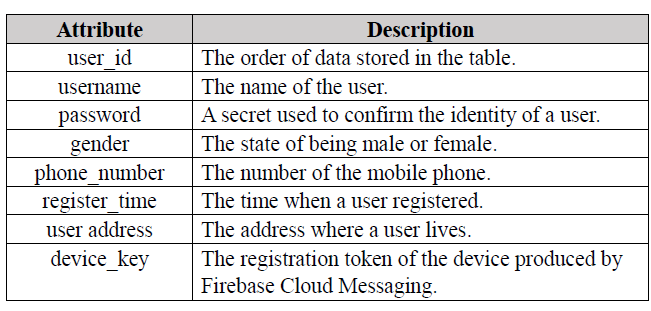
\includegraphics[width=0.85\textwidth]{./figures/Table3-1-UserTable.PNG}

\vspace{0.5cm}
\label{Fig:UserTable}
\end{figure}

 
The first table named user-table keeps the account information of registered users. Table 3.1 shows the data format of user-table. As mentioned in chapter 3.2.1, the attribute \textbf{"device\_key"} is the token generated by the application. The token is assigned to the mobile device rather than the user, and it will be updated when the user logins on different devices. Therefore, the SUMO server can know which device is bind to the user by the unique token. The attribute \textbf{"username"} is applied to identify the user who places the order. 

\begin{figure}[H]
\centering
\captionof{table}{\large County Table}
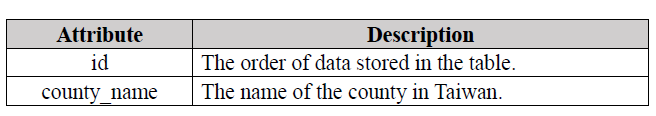
\includegraphics[width=0.85\textwidth]{./figures/Table3-2-CountyTable.PNG}
\vspace{0.5cm}
\label{Fig:CountyTable}
\end{figure}

\begin{figure}[H]
\centering
\captionof{table}{\large Township Table}
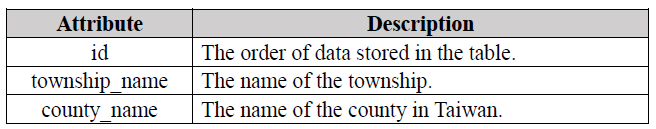
\includegraphics[width=0.85\textwidth]{./figures/Table3-3-TownshipTable.PNG}
\vspace{0.5cm}
\label{Fig:TownshipTable}
\end{figure}

The second table and the third table are county table and township table. The data format of the two tables is presented in Table 3.2, Table 3.3. The administrative district data of Taiwan is stored in the both tables. the data will be shown on the mobile application when the user wants to select the address of the shipper or receiver. Therefore, the typo can be reduced so that the process of geocoding can be performed better. 
The geocoding technology will be mentioned in Chapter 4. Furthermore, it provides scalability of service region, if the range of the simulation becomes larger, the administrator can easily expand regional options by adding additional data to the database. 

The last table is order table. As shown in Table 3.4, it retains information of the user’s order, and part of order will be explained in this section. The attribute \textbf{"status"} represents the situation of logistic activity, such as "on the way to the receiver’s address". 
In addition, it is the criteria whether if the receiver can designate the arrival time. The attribute \textbf{"sender\_name"} and \textbf{"receiver\_name"} are used by the SUMO server to determine users which the server will notify. The latitude and longitude transformed from senders’ address is stored as\textbf{ "sender\_lat"} and \textbf{“sender\_lng”}, and the same is true for the receiver’ address. The attribute \textbf{"sender\_time"} and\textbf{"receiver\_time"} are the expected arrival time that users select on the mobile application. The SUMO server will exploit the locational and time information to generate a dispatching schedule and arrange the route of each truck. 

\begin{figure}[H]
\centering
\captionof{table}{\large Order Table}
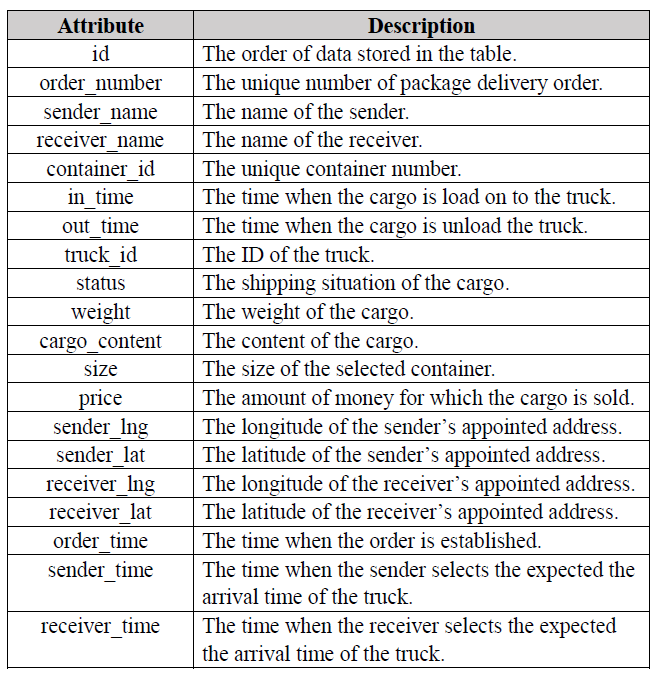
\includegraphics[width=0.85\textwidth]{./figures/Table3-4-OrderTable.PNG}
\vspace{0.5cm}
\label{Fig:OrderTable}
\end{figure}

  



\chapter{System Implementation}\label{Chap:System_Implementation}

\section{Mobile Application}


Among all mobile operating systems, Android OS holds 86.7\% market share according to the survey.[] It is the most widely-used operating system in the world. Given that the self-driving delivery will be popularized in all walks of life soon after, Android OS is the most suitable system for developmentthe mobile application. The application is built by the Android Software Development Kit (Android SDK), and it is developed on Android Studio which is Integrated Development Environment for Android. Android Studio provides a preview of the user interface and it has the built-in support of Google Cloud Platform. Consequently, it is an appropriate way to construct the mobile application of the system. Furthermore, Google Map SDK for Android and Google Geocoding API were added to the mobile application, the former enables the application to display the map of simulation and mark the address, the latter is able to transform the street address into latitude and longitude.

\begin{figure}[H]
\centering
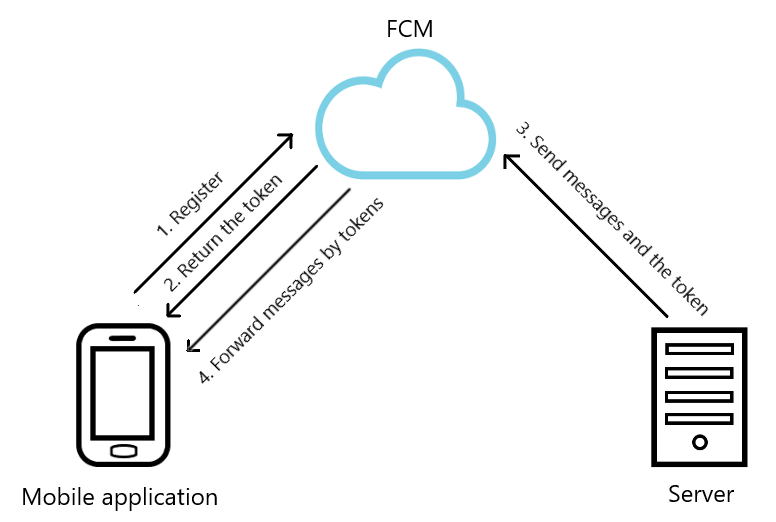
\includegraphics[width=1.0\textwidth]{./figures/F4-1_FCM.PNG}
\caption{\large Firebase Cloud Messaging.}
\vspace{0.5cm}
\label{Fig:FCM}
\end{figure}

In order to send the messages to notify the users that the truck has arrived to the destination, a cloud solution for messages and notifications is included in the self-driving delivery system. Firebase Cloud Messaging (FCM) is a service provided by Firebase, which is a subsidiary of Google, and it facilitates messaging between the mobile application and the server built by developers. 

As illustrated in Figure 4.1, there are three components such as mobile application, FCM, and the server. The mobile application involves in the process of message passing.
FCM and the server that intends to send notifications (i.e., TraCI server in this thesis). 
When the mobile application is installed on the mobile device and launched for the first time, the apps will send a registration request to FCM through FCM SDK. Then, the FCM server will generate a corresponding token for the device, and return the token back to the mobile application. The token would be uploaded to the database if users log in. Conversely, when users log out, the token in the database will be removed to prevent the server from notifying the wrong users. According to the tokens stored in the FCM server, the messages sent from the TraCI (Traffic Control Interface) server will be forwarded to the appointed device by FCM.


The initialization of user interface in the mobile application is illustrated in Figure 4.2. As shown in Figure 4.2a, the homepage of the application is constituted by the buttons of the main functions. the study develops a simple registration function of a user account, which is shown in Figure 4.2b. 
Before a user logs in, the FCM token is stored in the memory of the device. The user can be distinguished in different mobile devices with the unique token after logging in.
 




\begin{figure}[H]
\centering  %图片全局居中
\subfigure[Home Page.]{
\label{Fig.sub.1}
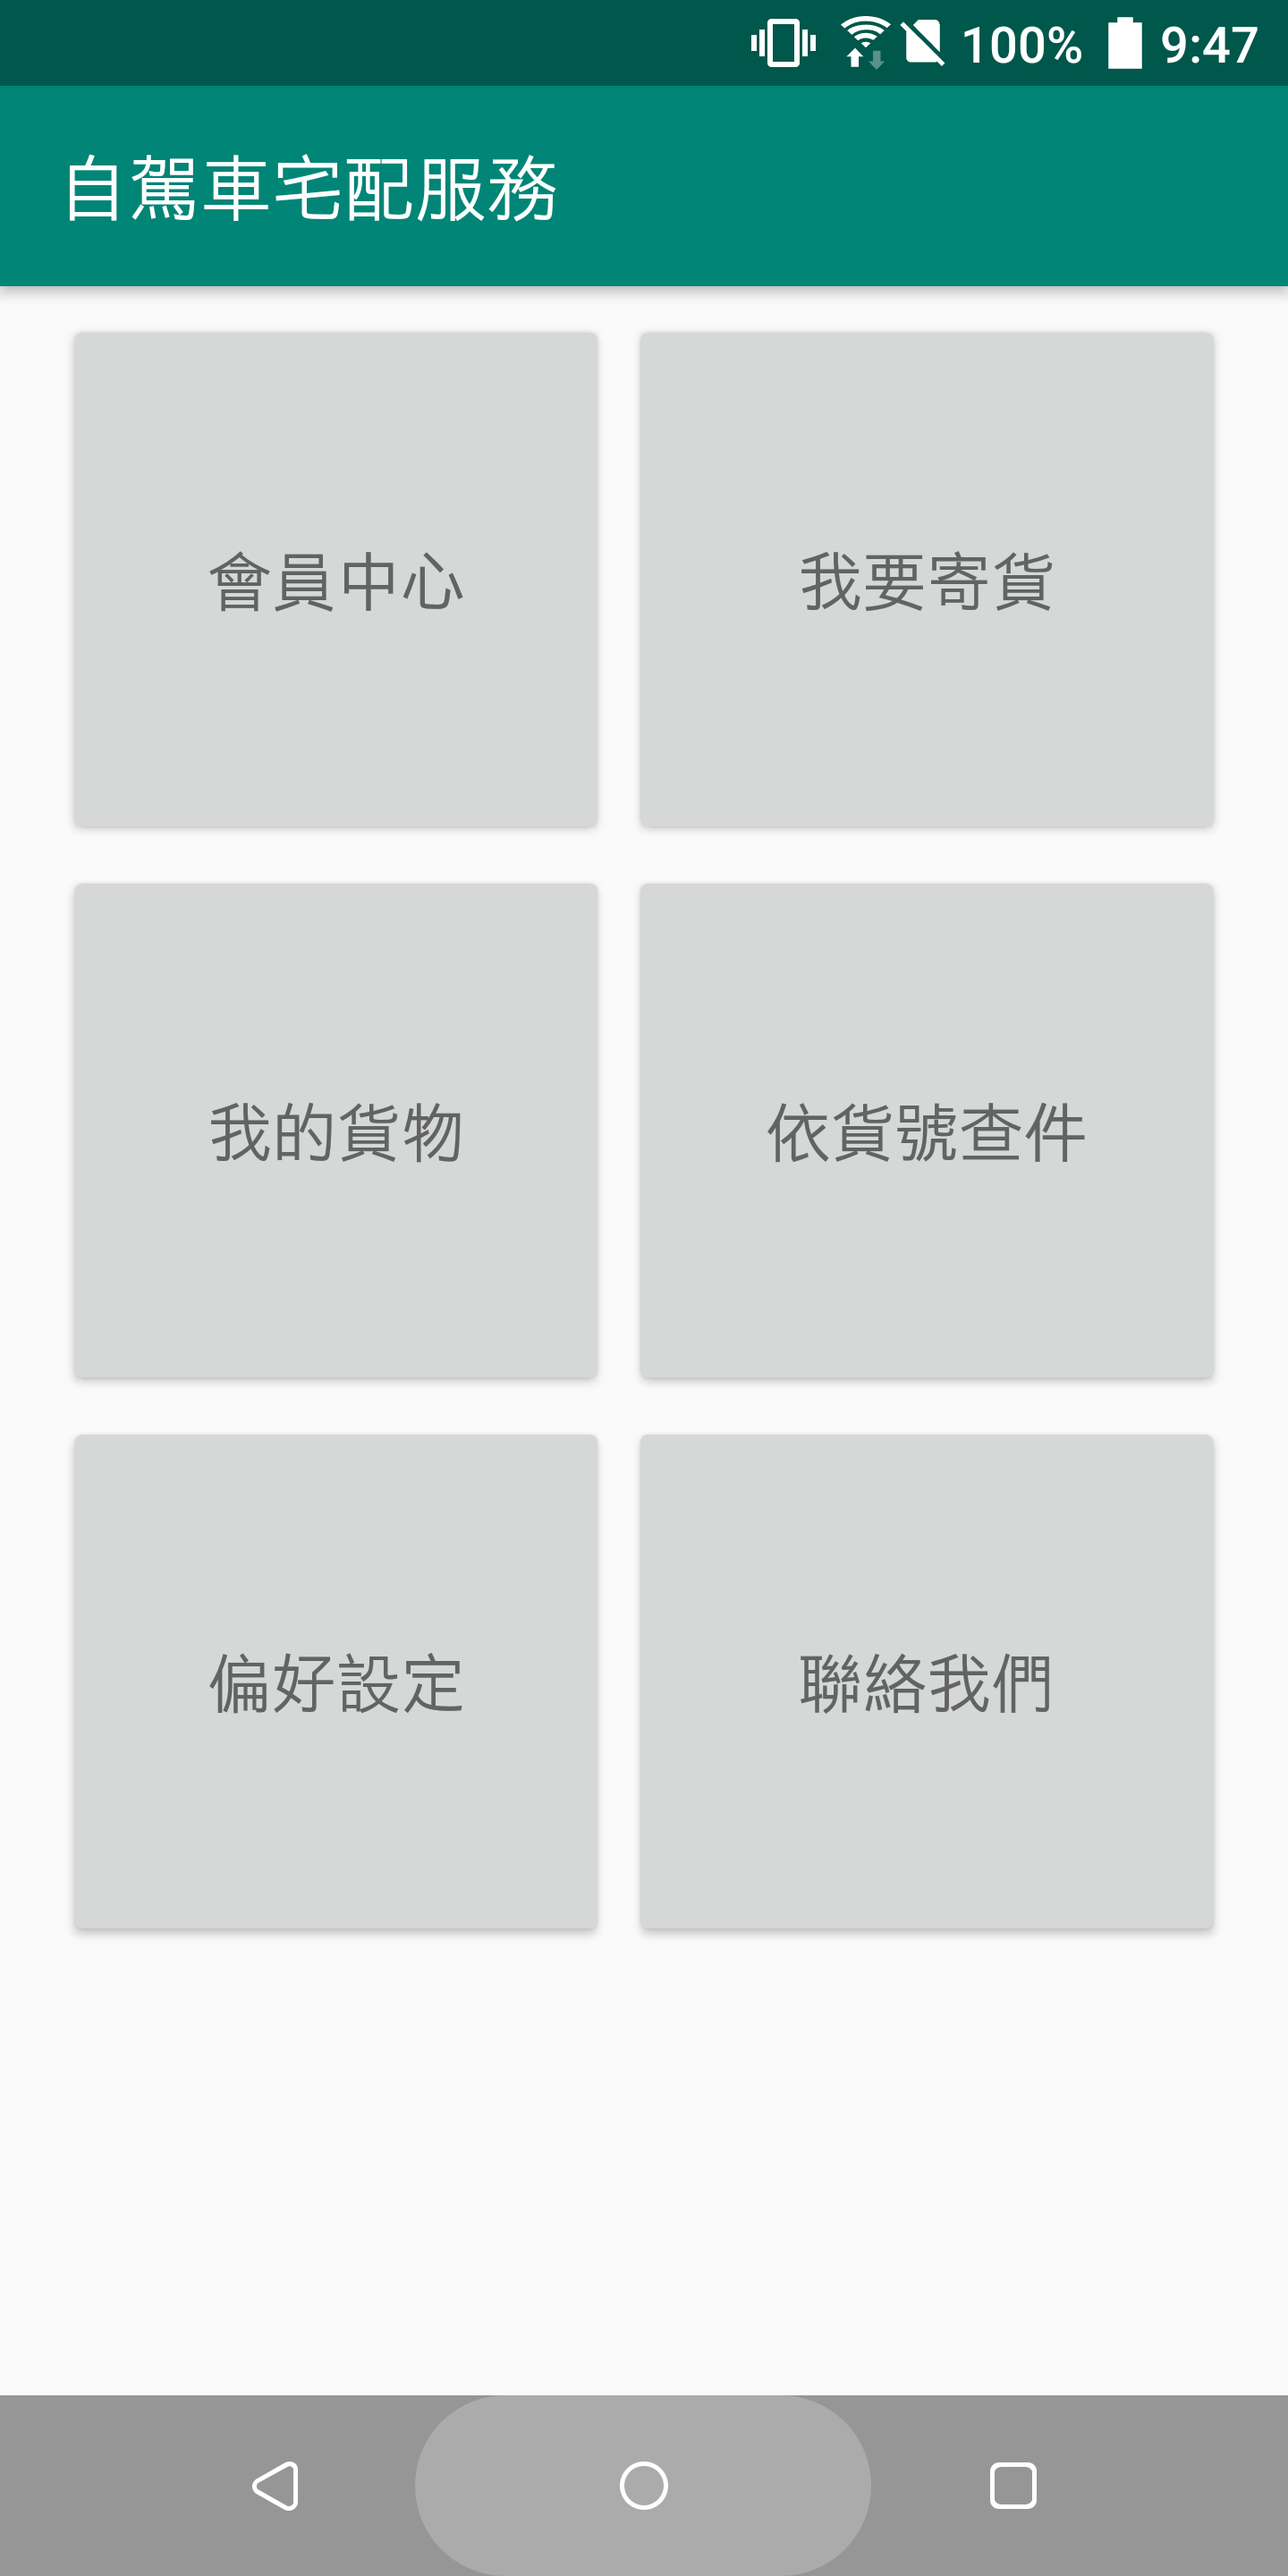
\includegraphics[width=0.45\textwidth]{./figures/F4-2-a-HomePage.PNG}
}
\subfigure[Login.]{
\label{Fig.sub.2}
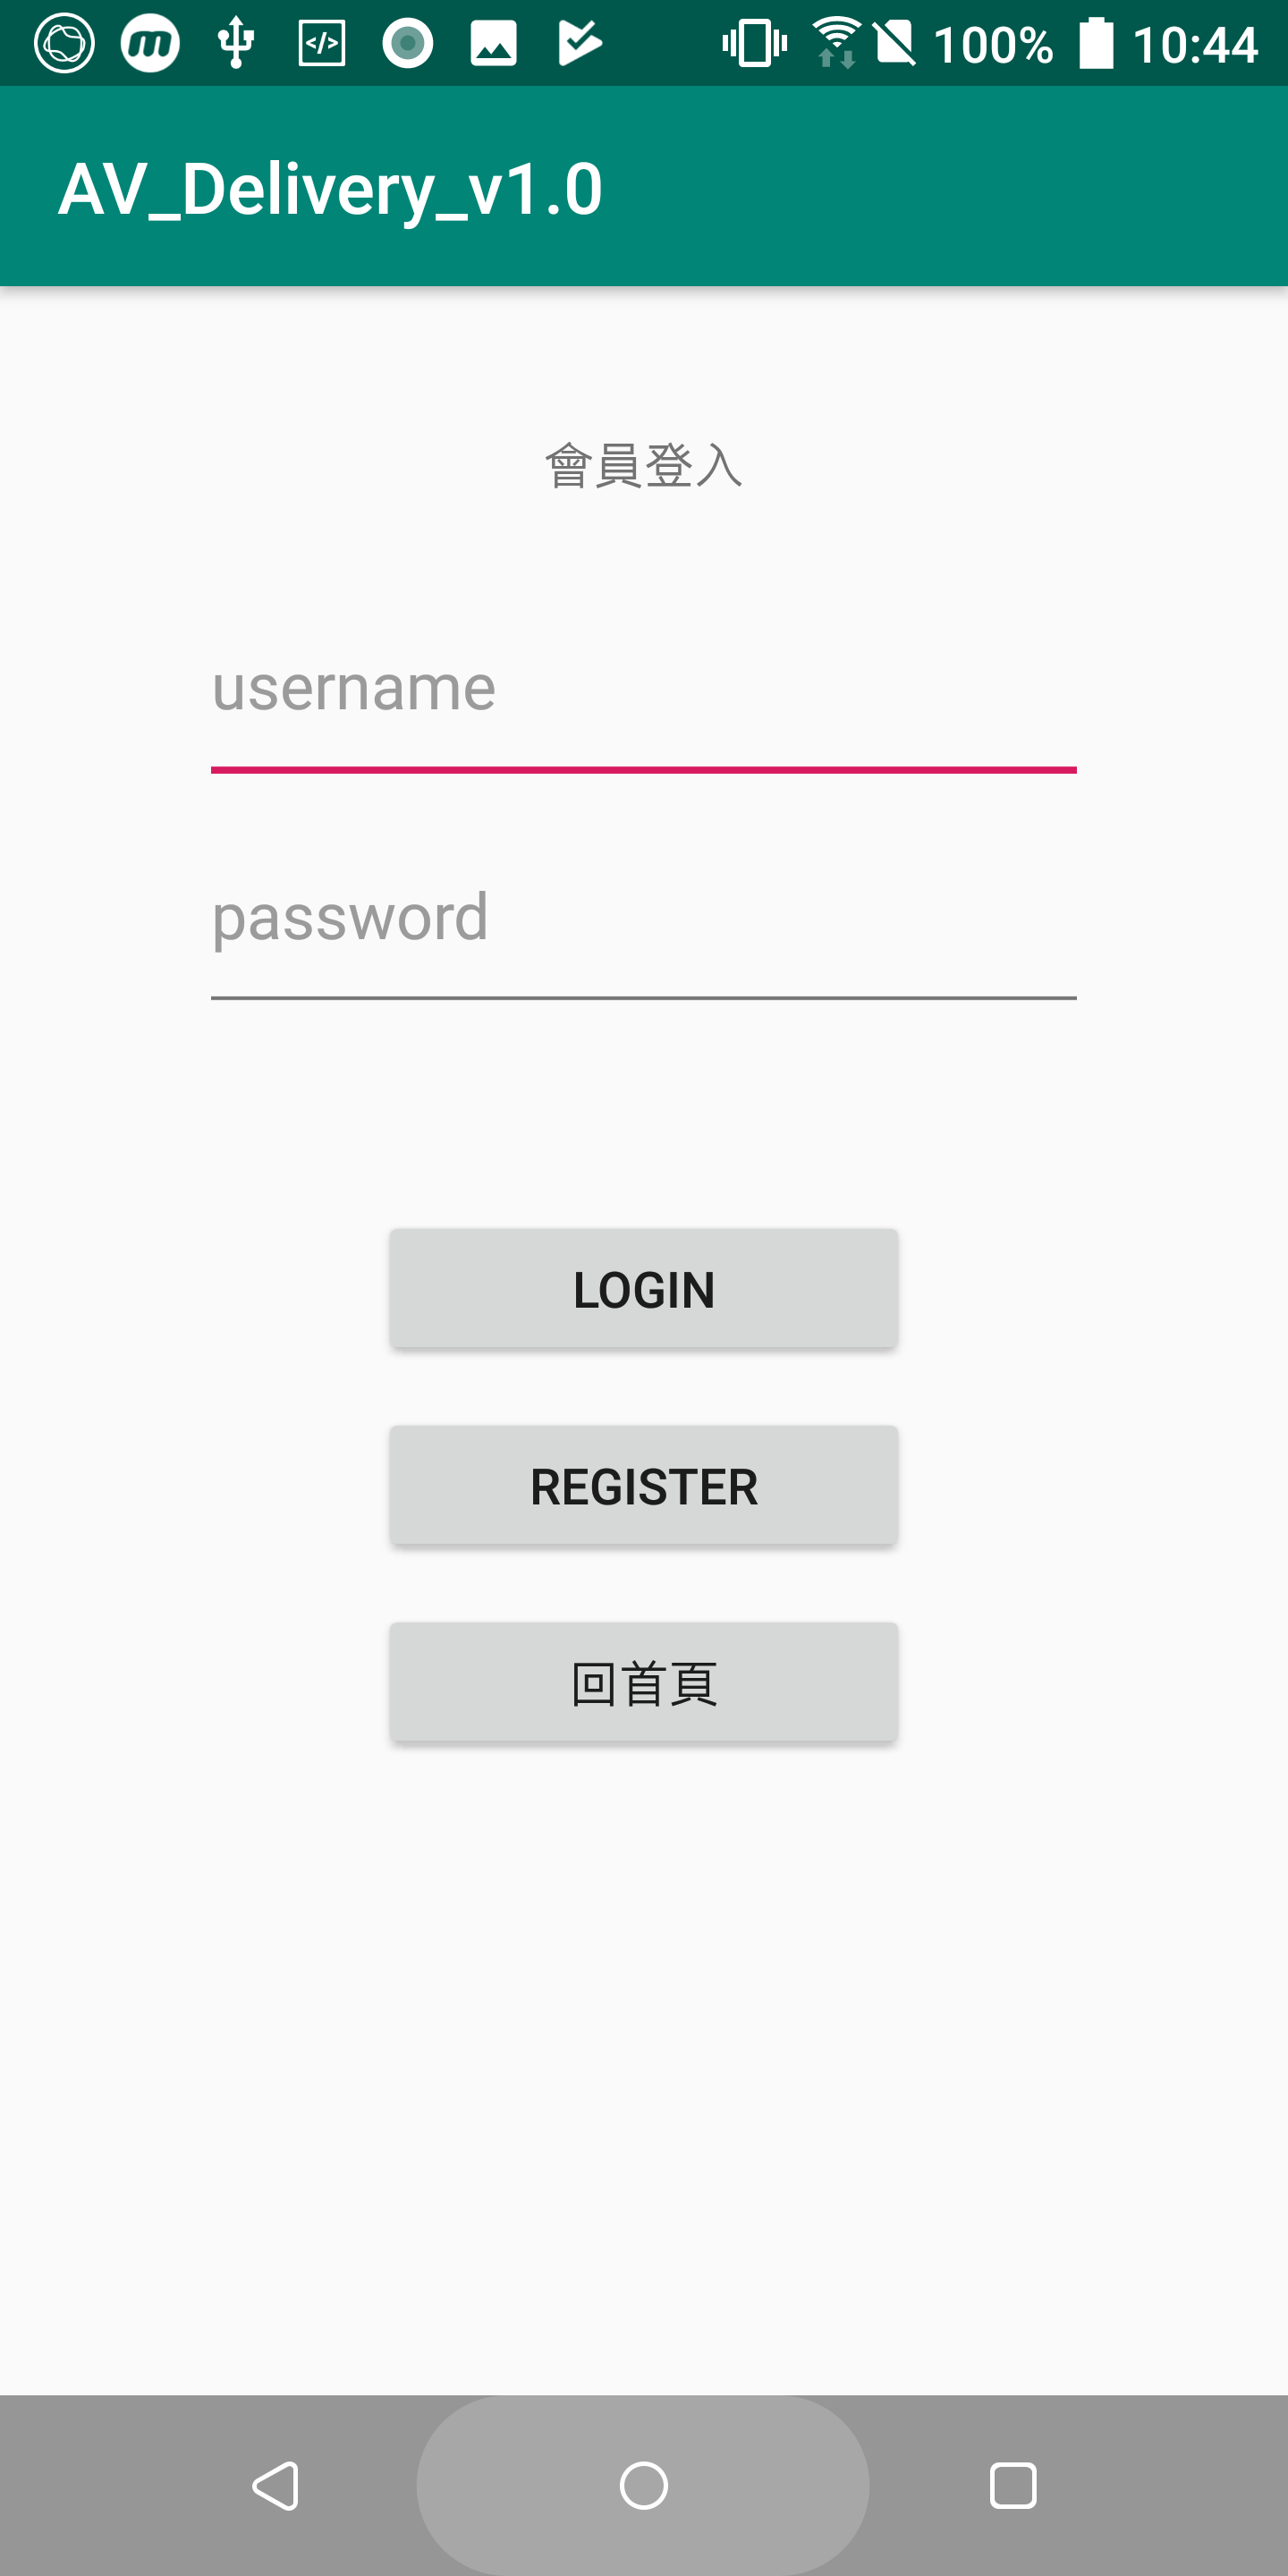
\includegraphics[width=0.45\textwidth]{./figures/F4-2-b-Login.PNG}}

\caption{Initialization of the user interface.}
\label{Initialization_of_UserInterface}
\end{figure}

Figure 4.3 depicts the page of placing a package delivery order, the user must fill in all the fields of the order. The option of container size can be expanded based on the container type of the logistics companies.

\begin{figure}[H]
\centering
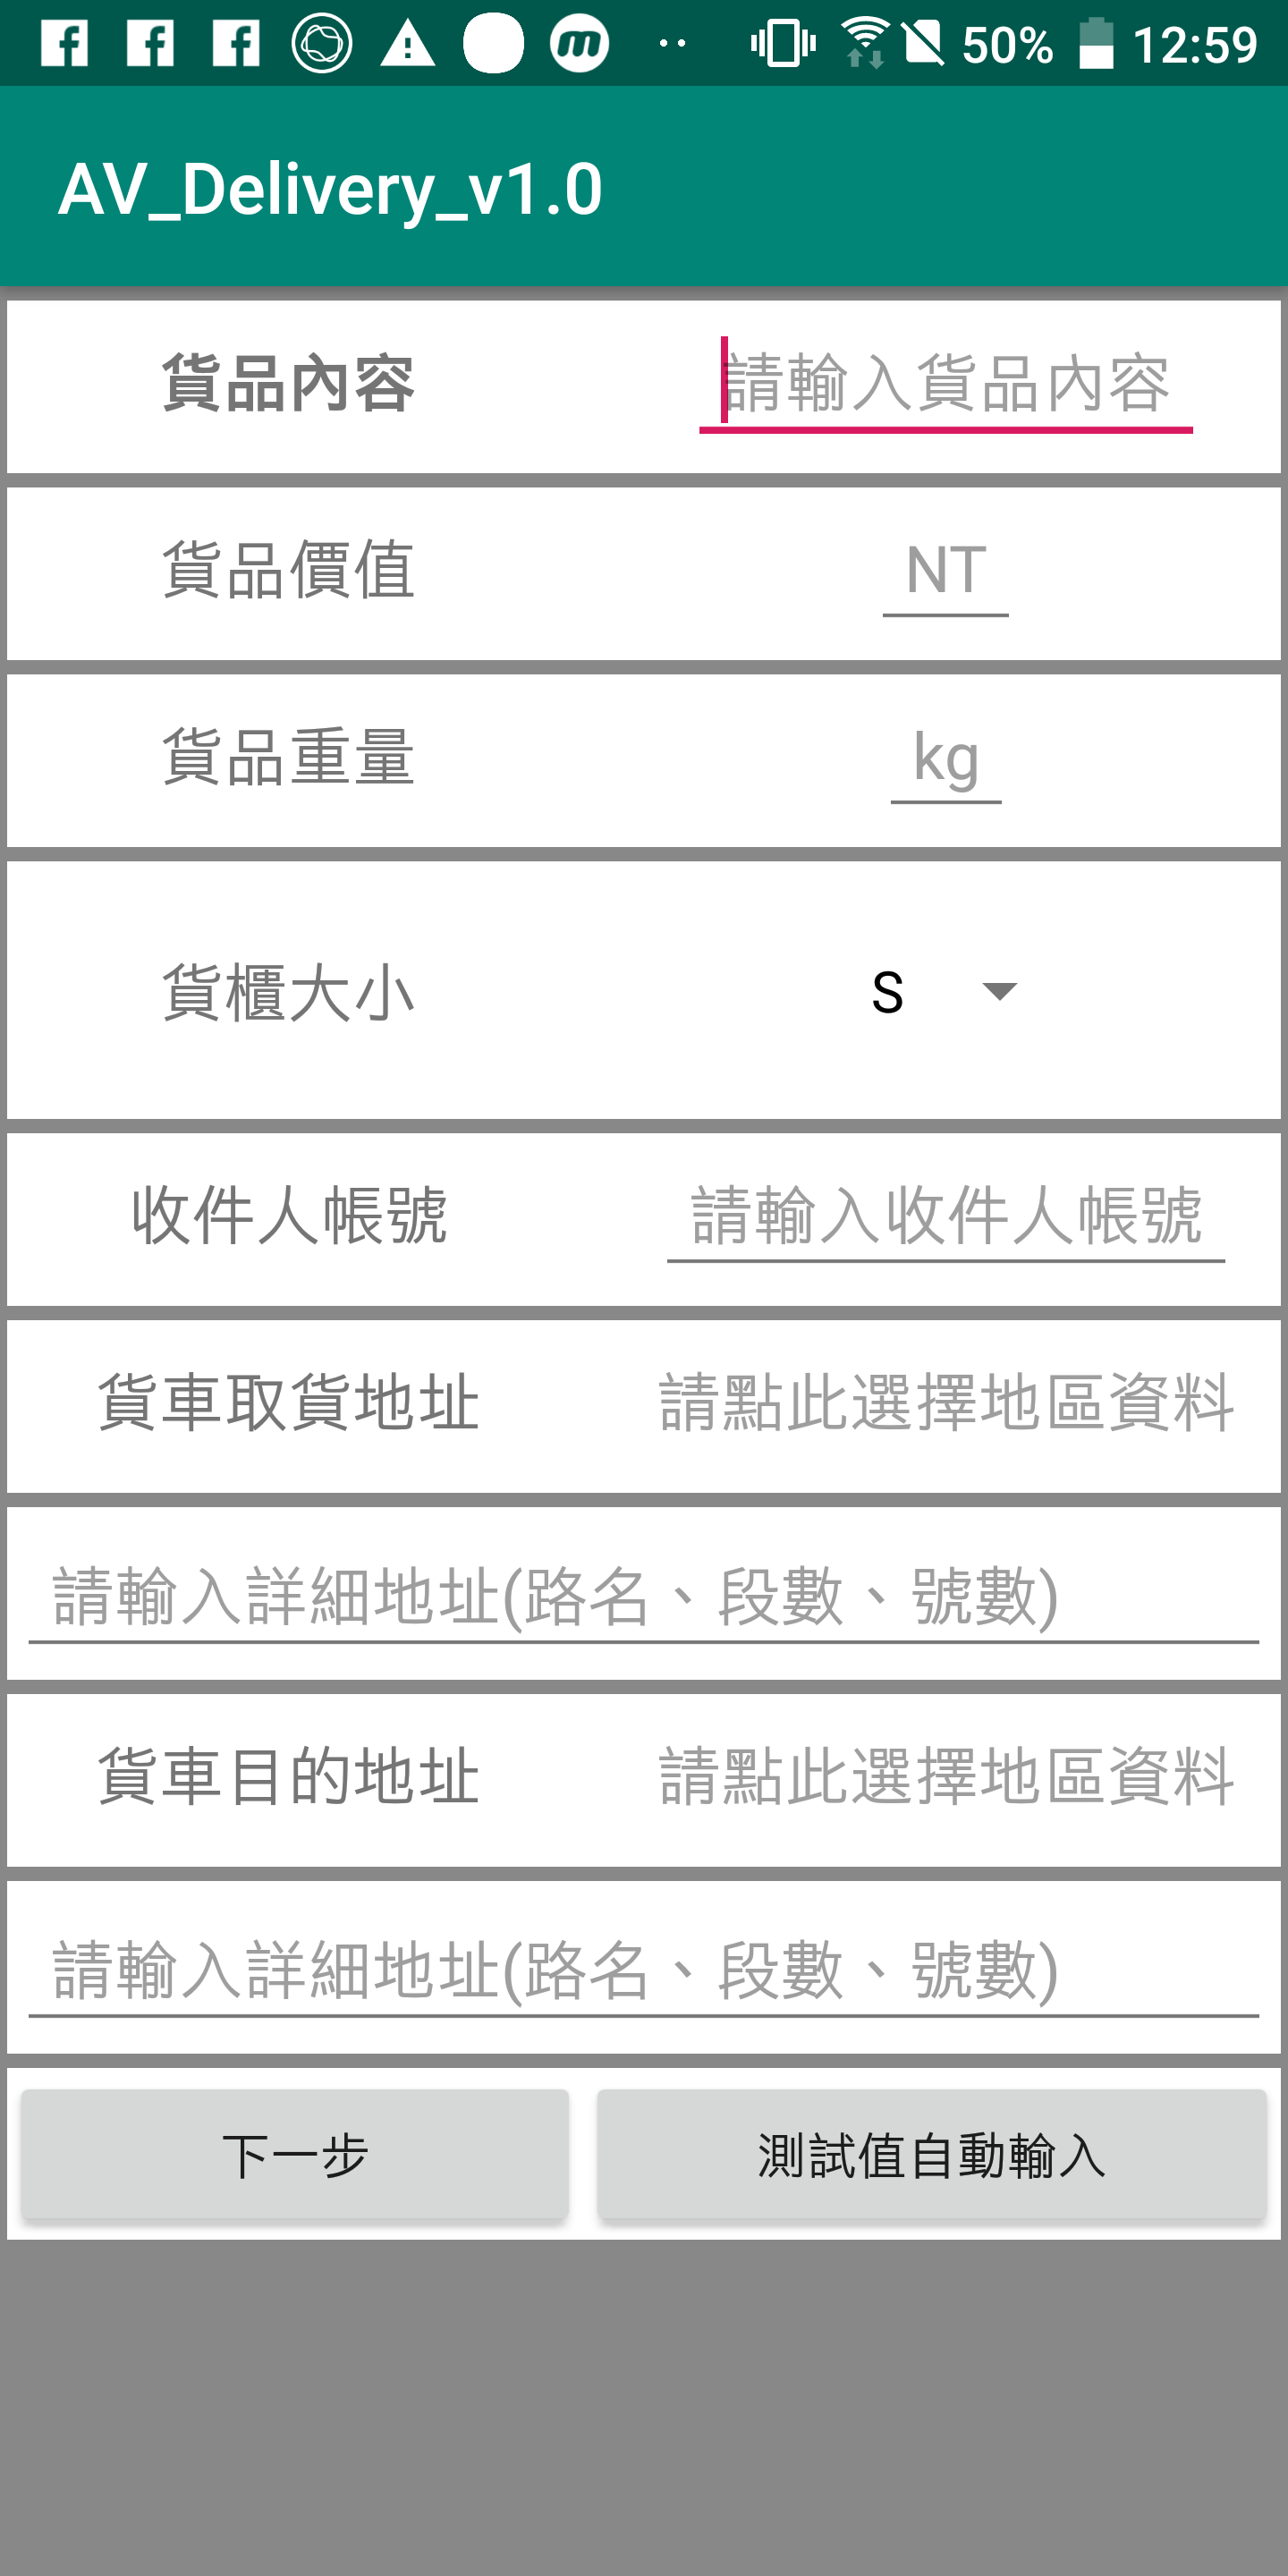
\includegraphics[scale=0.125]{./figures/F4-3-Place_an_order.PNG}
\caption{\large Place an order.}
\vspace{0.5cm}
\label{Fig:Place_an_order}
\end{figure}


The user can press the \textbf{region selecting button} to get the administrative district of the simulation range, which is shown in Figure 4.4. This function make the user input data faster and reduce the typing errors. The simulation region contains parts of the downtown areas in Tainan City. 


\begin{figure}[H]
\centering  %图片全局居中
\subfigure[City selection.]{
\label{Fig.sub.1}
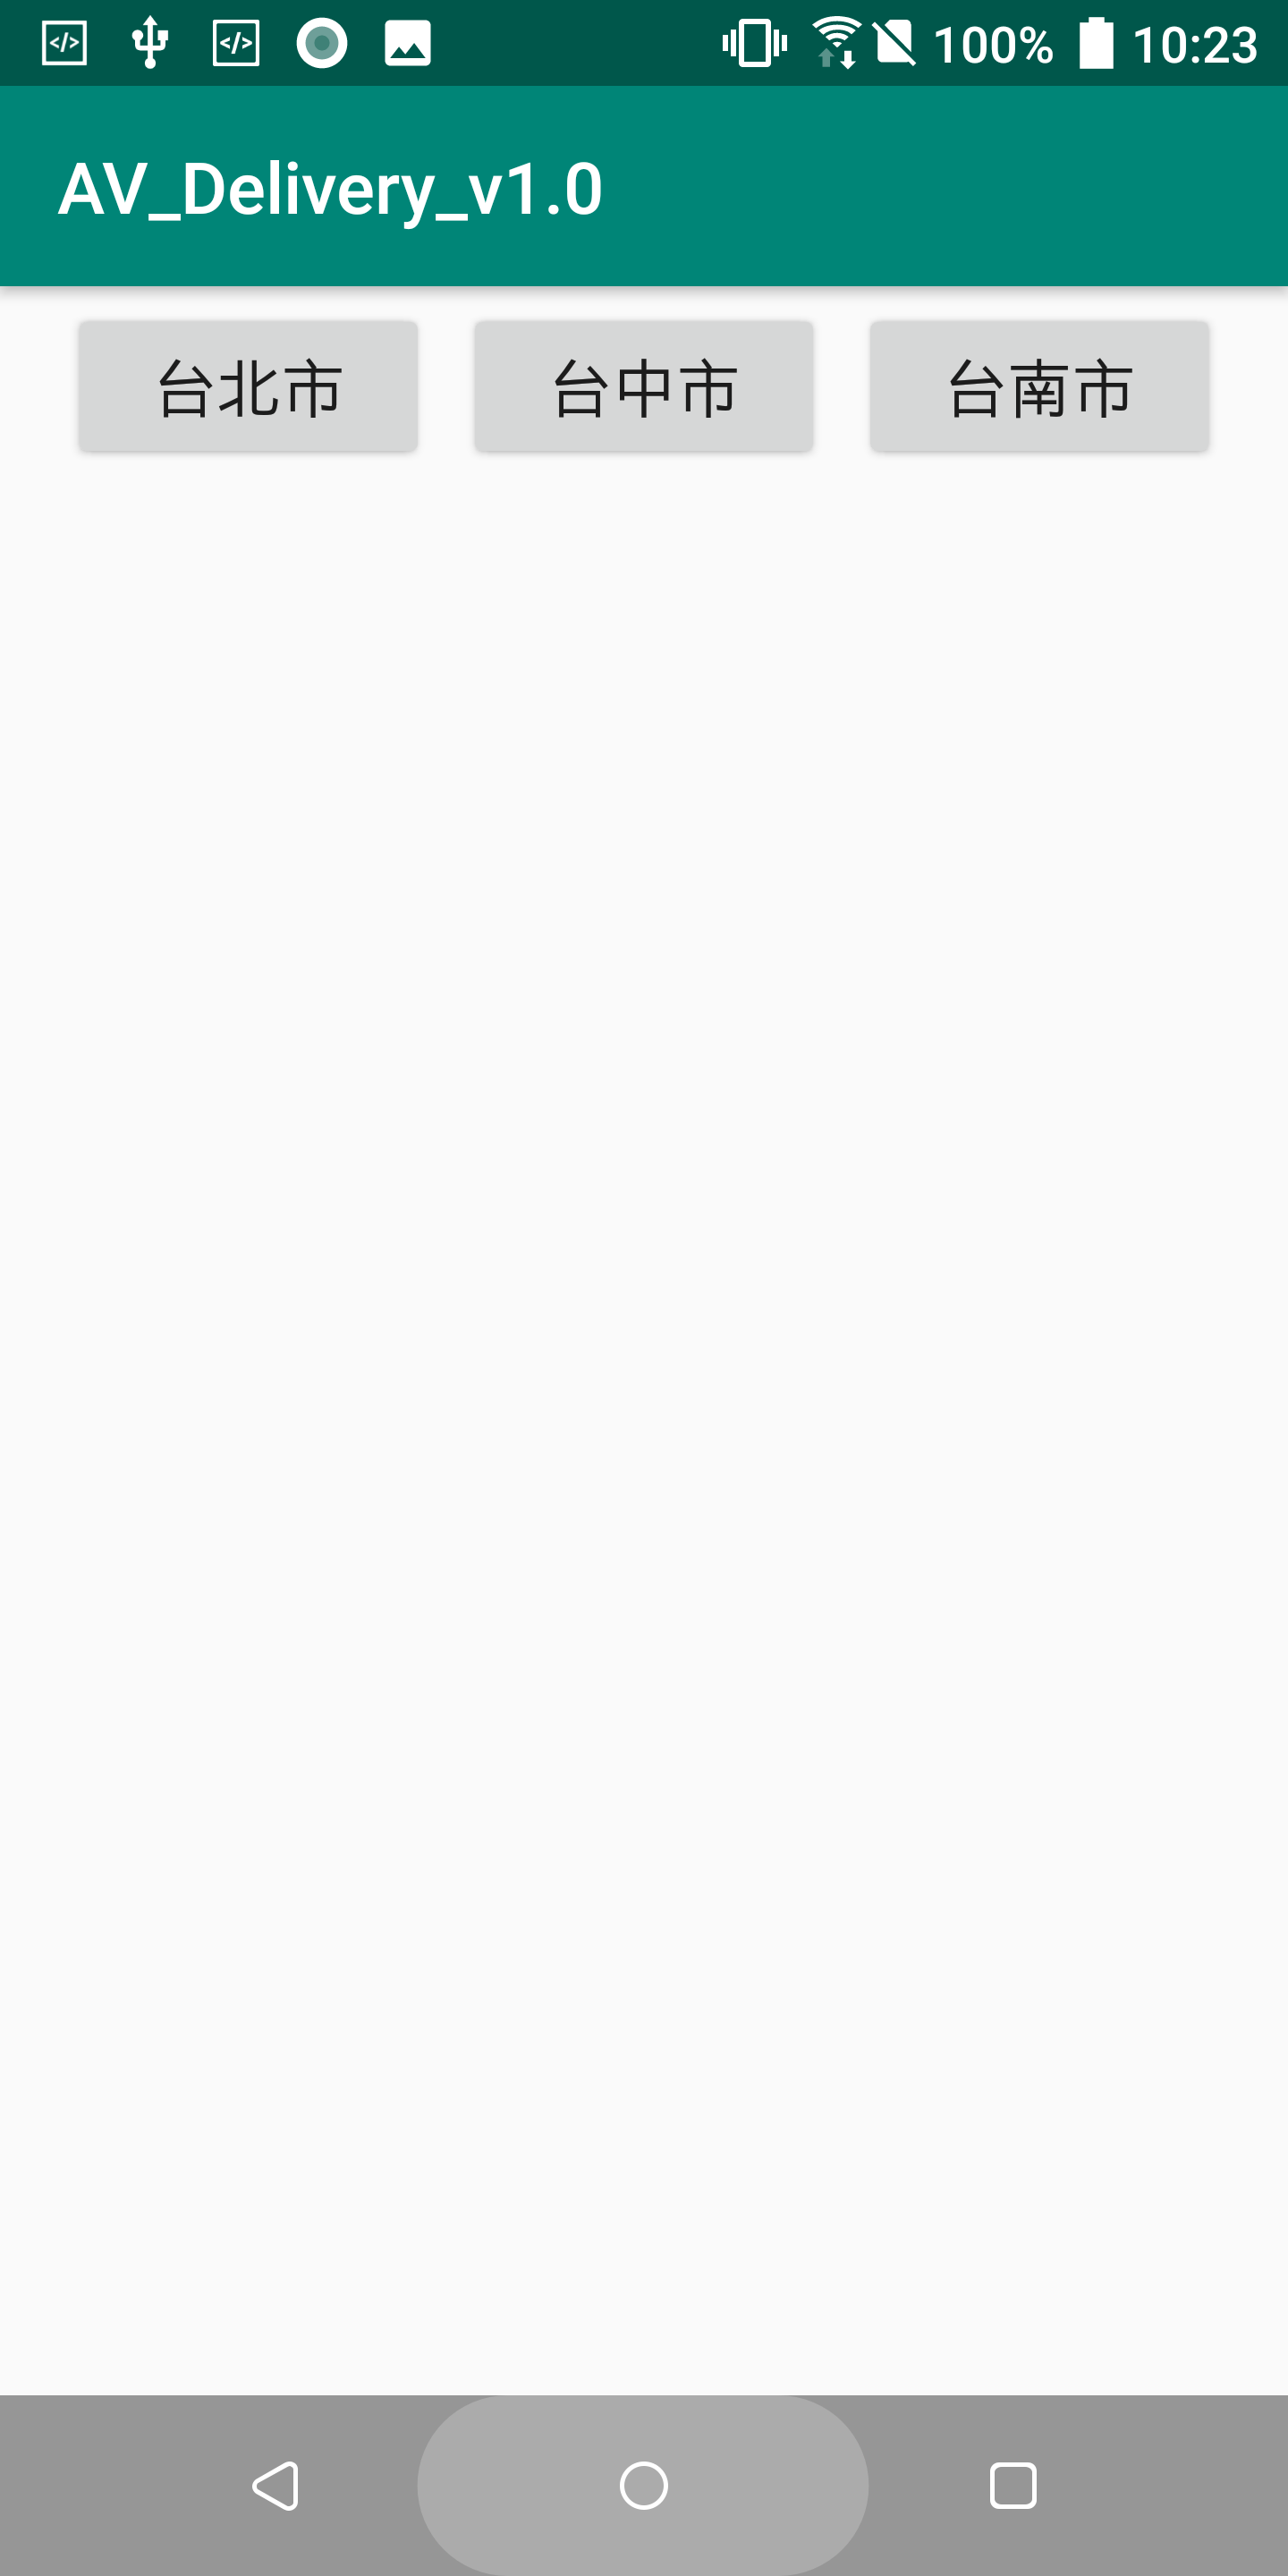
\includegraphics[width=0.45\textwidth]{./figures/F4-4-a-CitySelection.PNG}
}
\subfigure[District selection.]{
\label{Fig.sub.2}
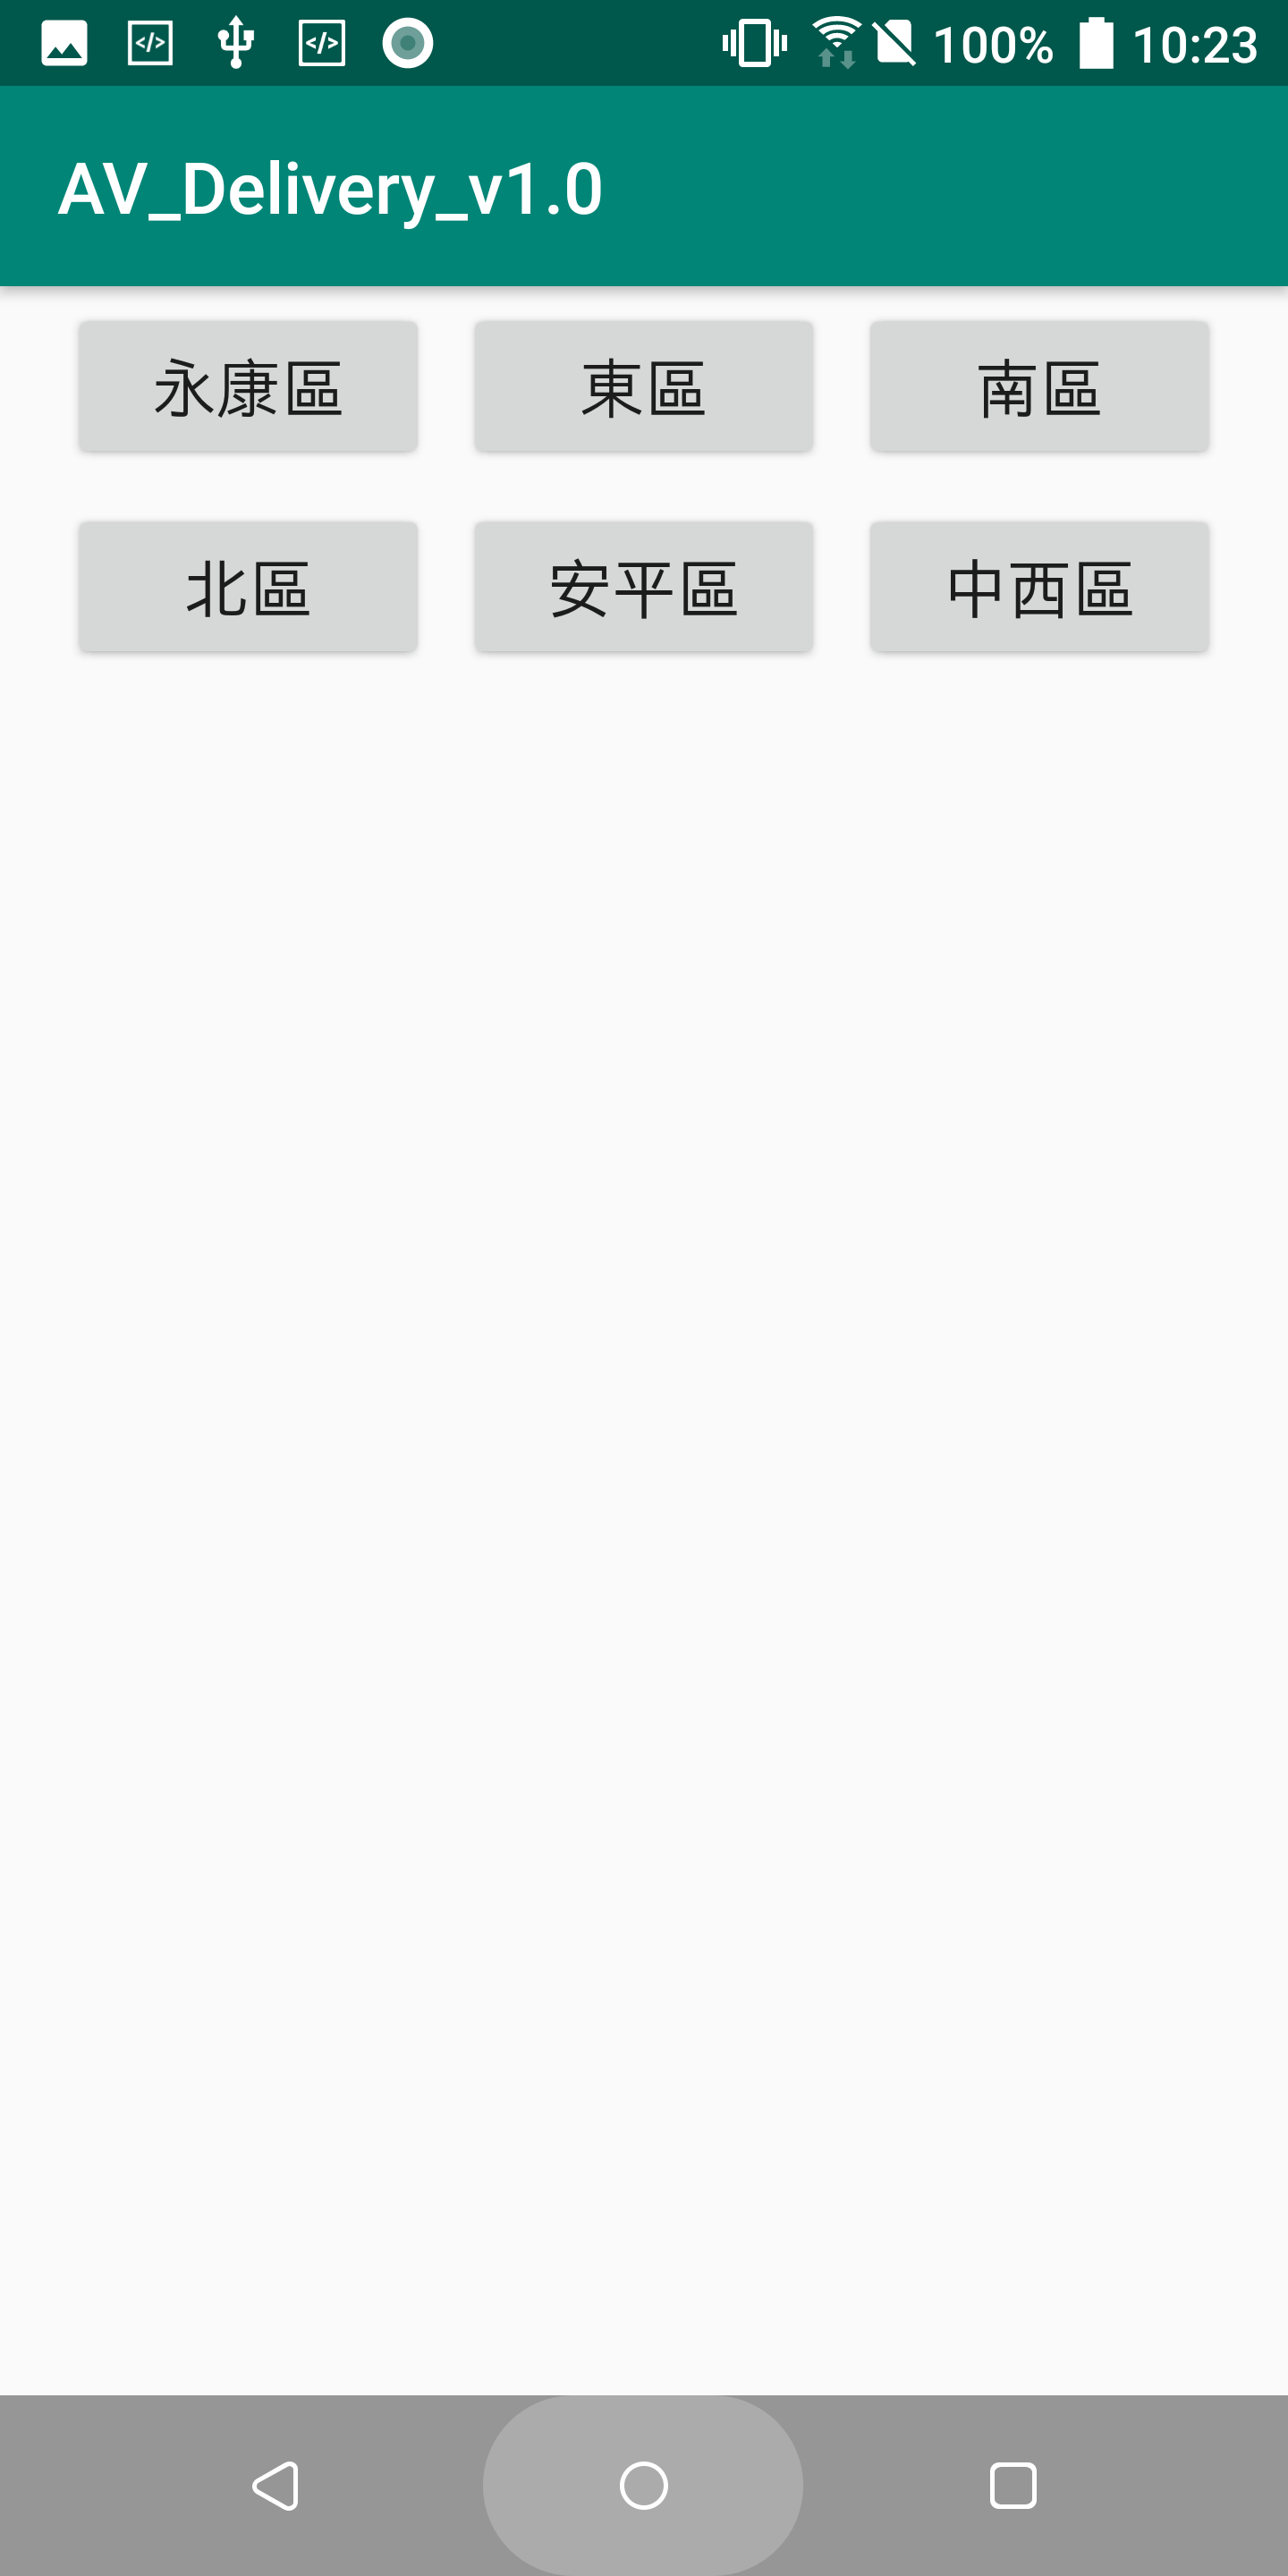
\includegraphics[width=0.45\textwidth]{./figures/F4-4-b-DistrictSelection.PNG}}

\caption{Region selection.}
\label{Region_selection}
\end{figure}


For the sake of convenience, the application will record the data entered by the user last time, and the data will be filled in the order automatically when clicking the auto inputting button. After filling out the order information, the user can press the next button, and the application would check whether the user name of receiver exist.

\begin{figure}[H]
\centering
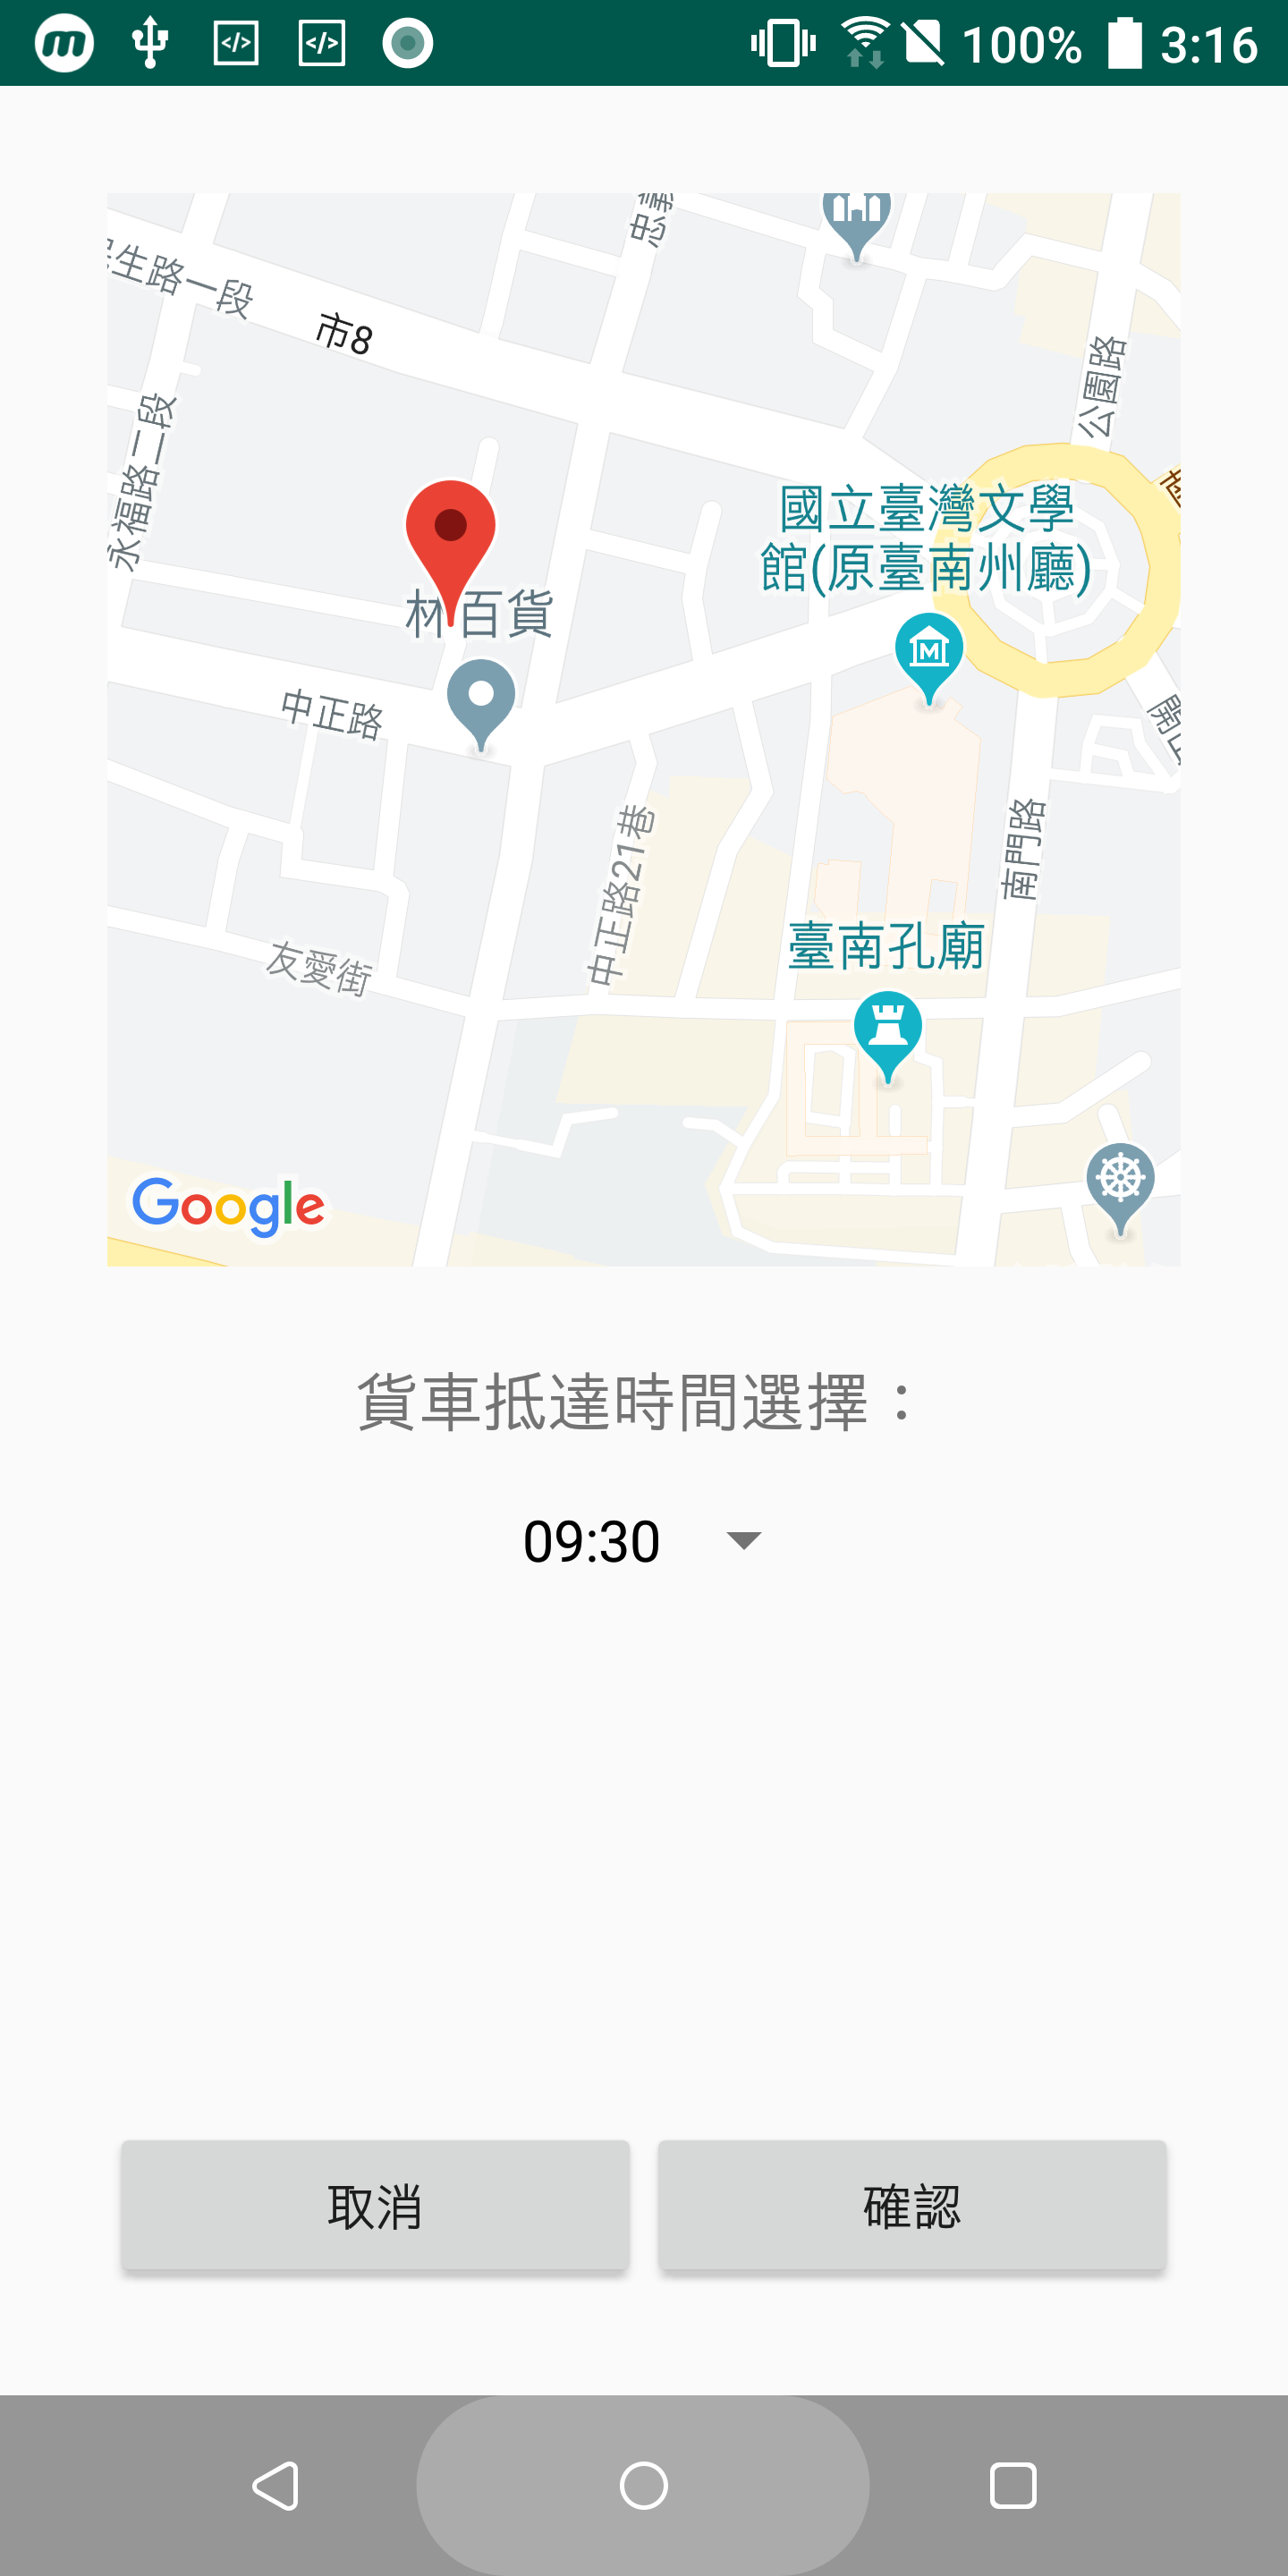
\includegraphics[scale=0.125]{./figures/F4-5-Localization.PNG}
\caption{\large Localization of the destination.}
\vspace{0.5cm}
\label{Fig:localization_of_destination}
\end{figure} 

As illustrated in Figure 4.5, the address that the user input will be transform into geographic location, and the shipper’s address will be displayed on the Google Map so that the user can confirm if the localization is correct. Then, the user can use the dropdown list to select the arrival time of the truck. 
Finally, the order request will be sent to the SUMO server by socket program. If there are eligible trucks in the simulated environment, the server would return a success message. Otherwise, the page will not be closed, and the user can choose other expected arrival time.  

\begin{figure}[H]
\centering  %图片全局居中
\subfigure[The packages I sent.]{
\label{packages_I_sent}
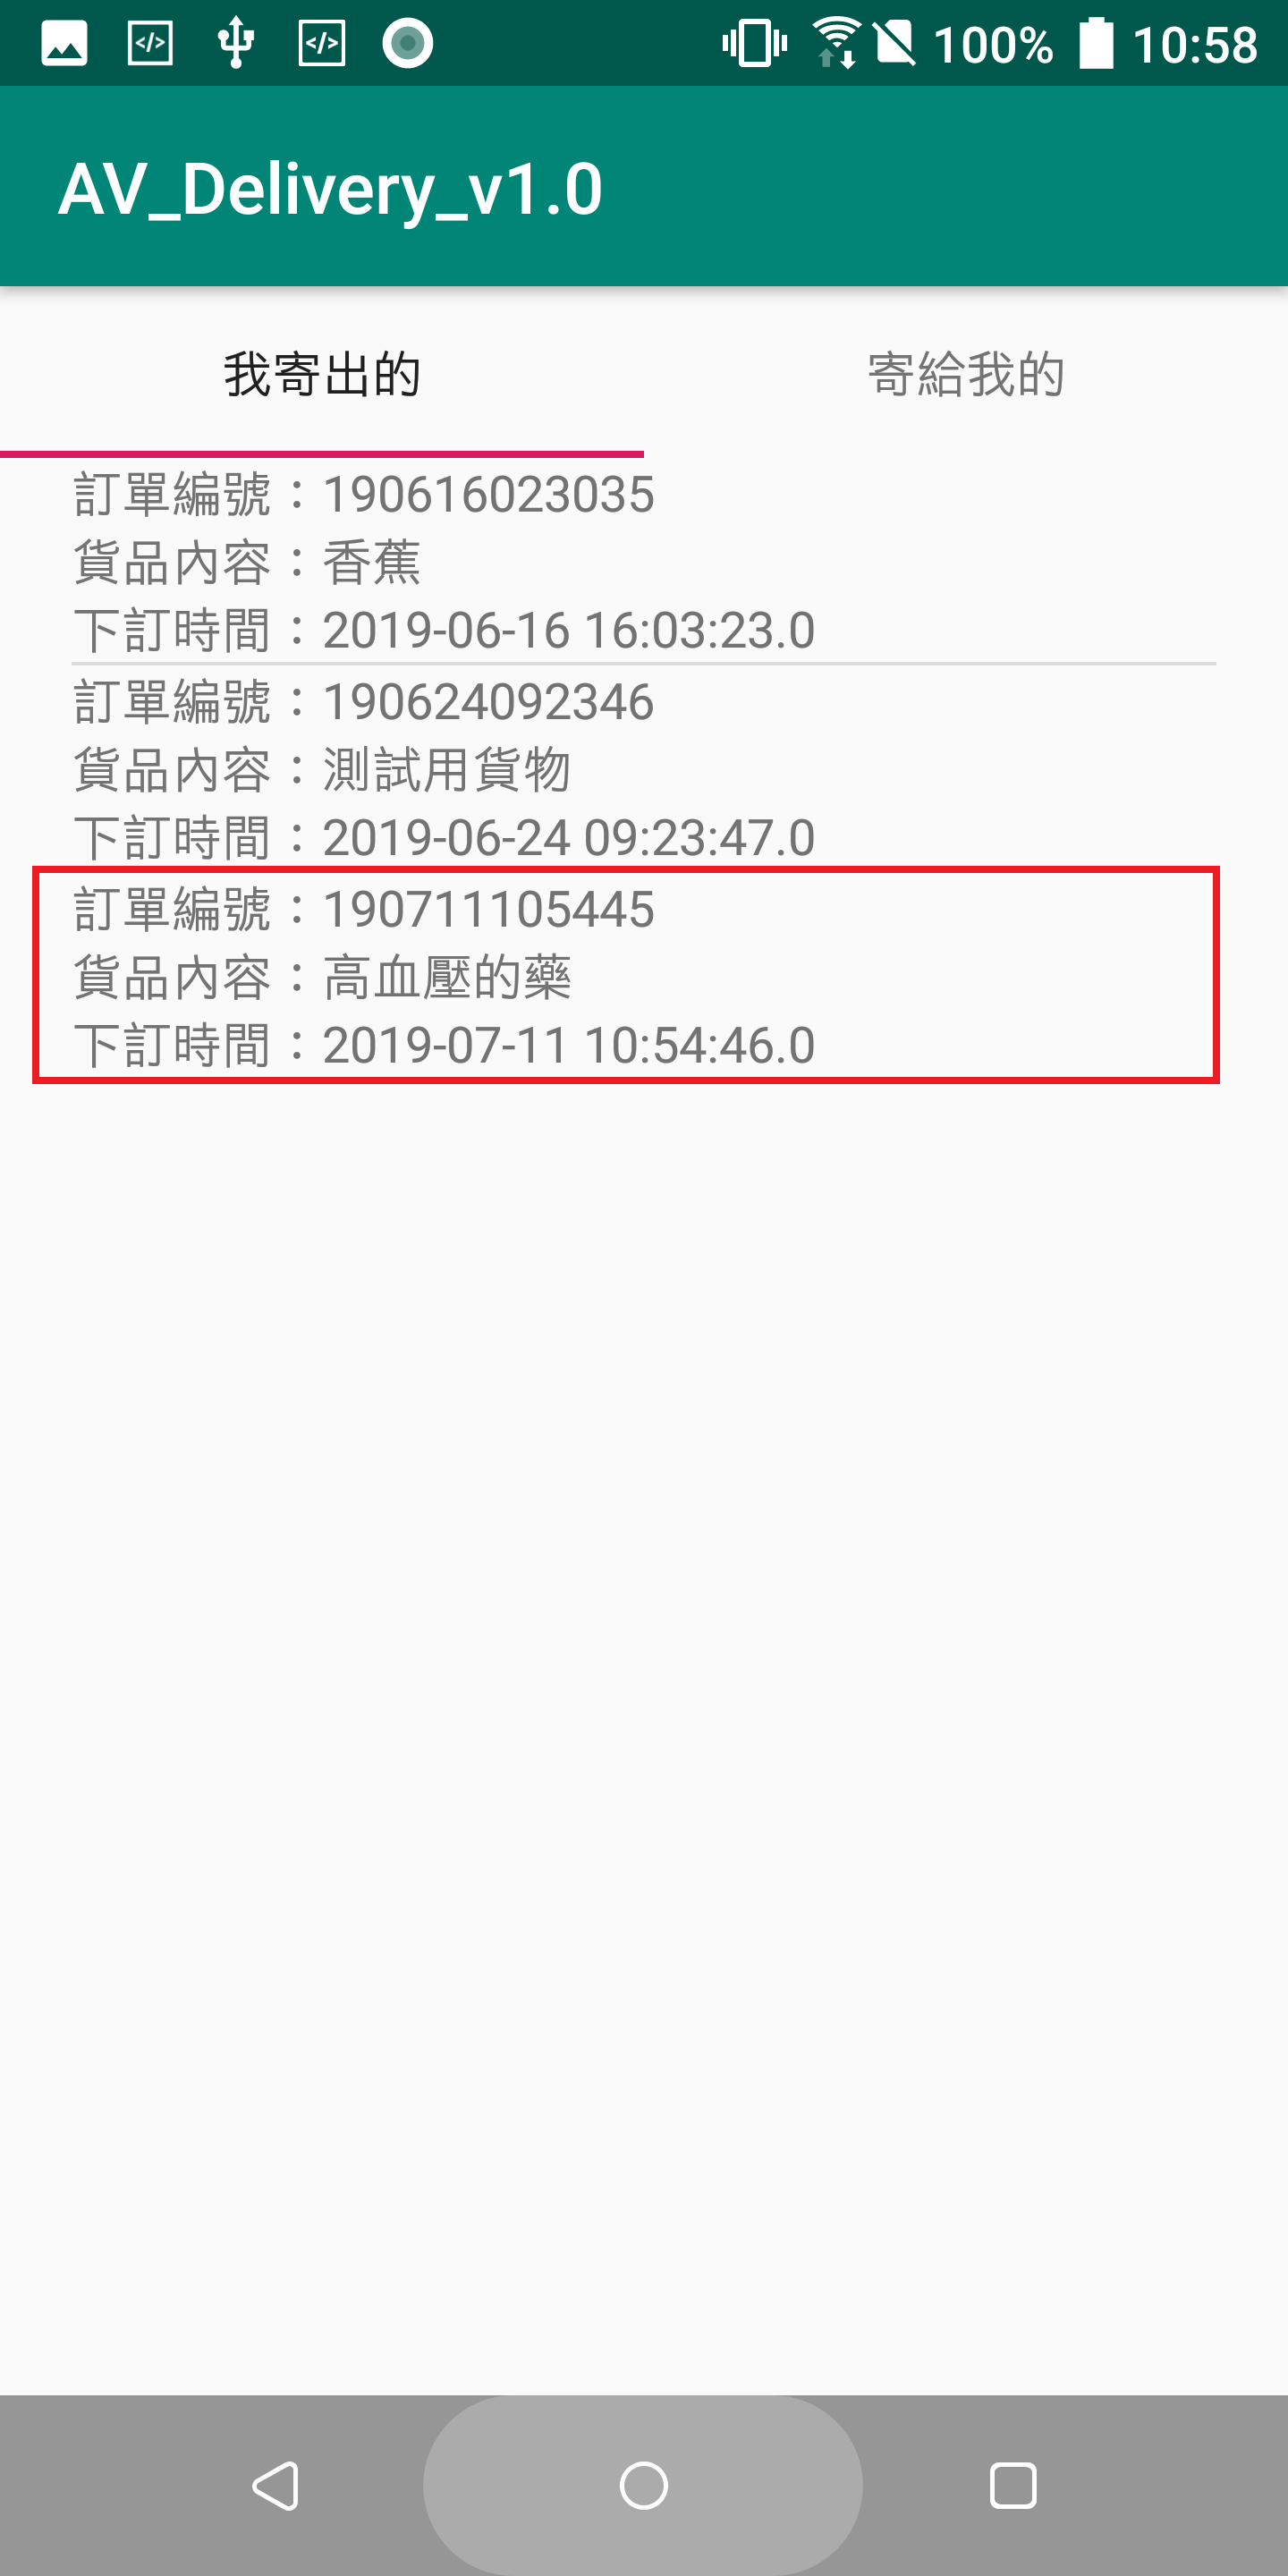
\includegraphics[width=0.45\textwidth]{./figures/F4-6-a-Package_I_sent.PNG}
}
\subfigure[The packages I received.]{
\label{packages_I_sent}
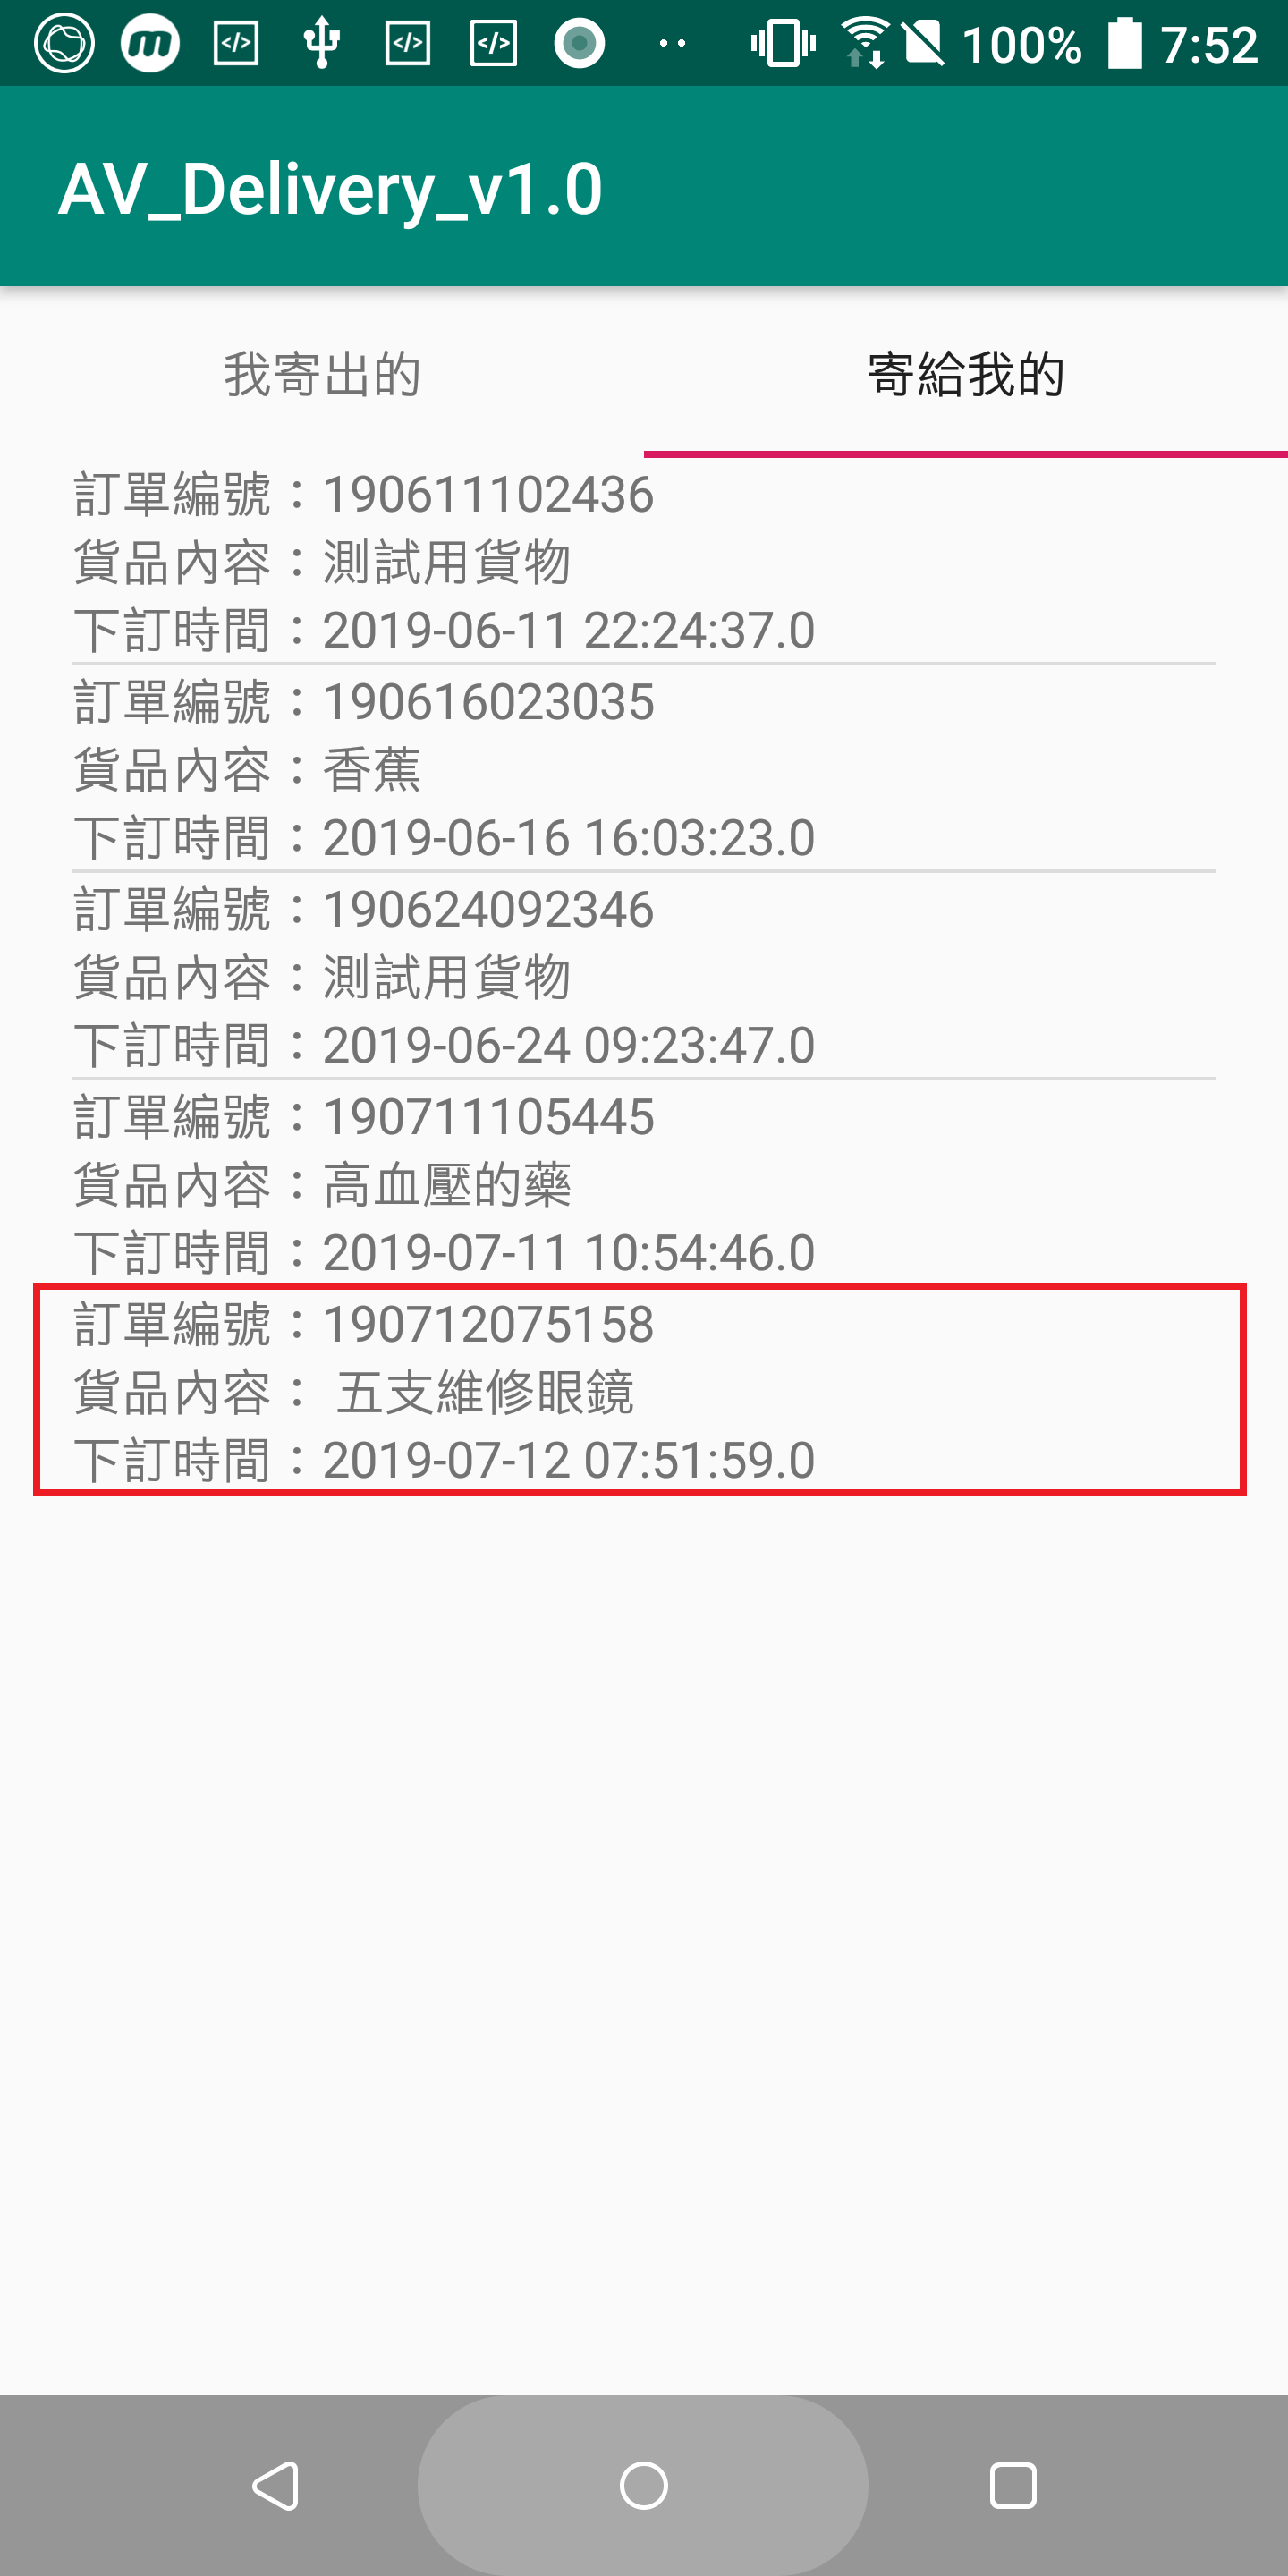
\includegraphics[width=0.45\textwidth]{./figures/F4-6-b-Package-I-received.PNG}}

\caption{Tracking history orders.}
\label{Tracking_history_orders}
\end{figure}

The established order can be viewed on the page of tracking orders shown in Figure 4.6.  This page has two cases. First case is to check the parcels the user sent. After sliding the tab above the page, the user switches into the second case. The second case is to examine the history packages which the user received.

\begin{figure}[H]
\centering
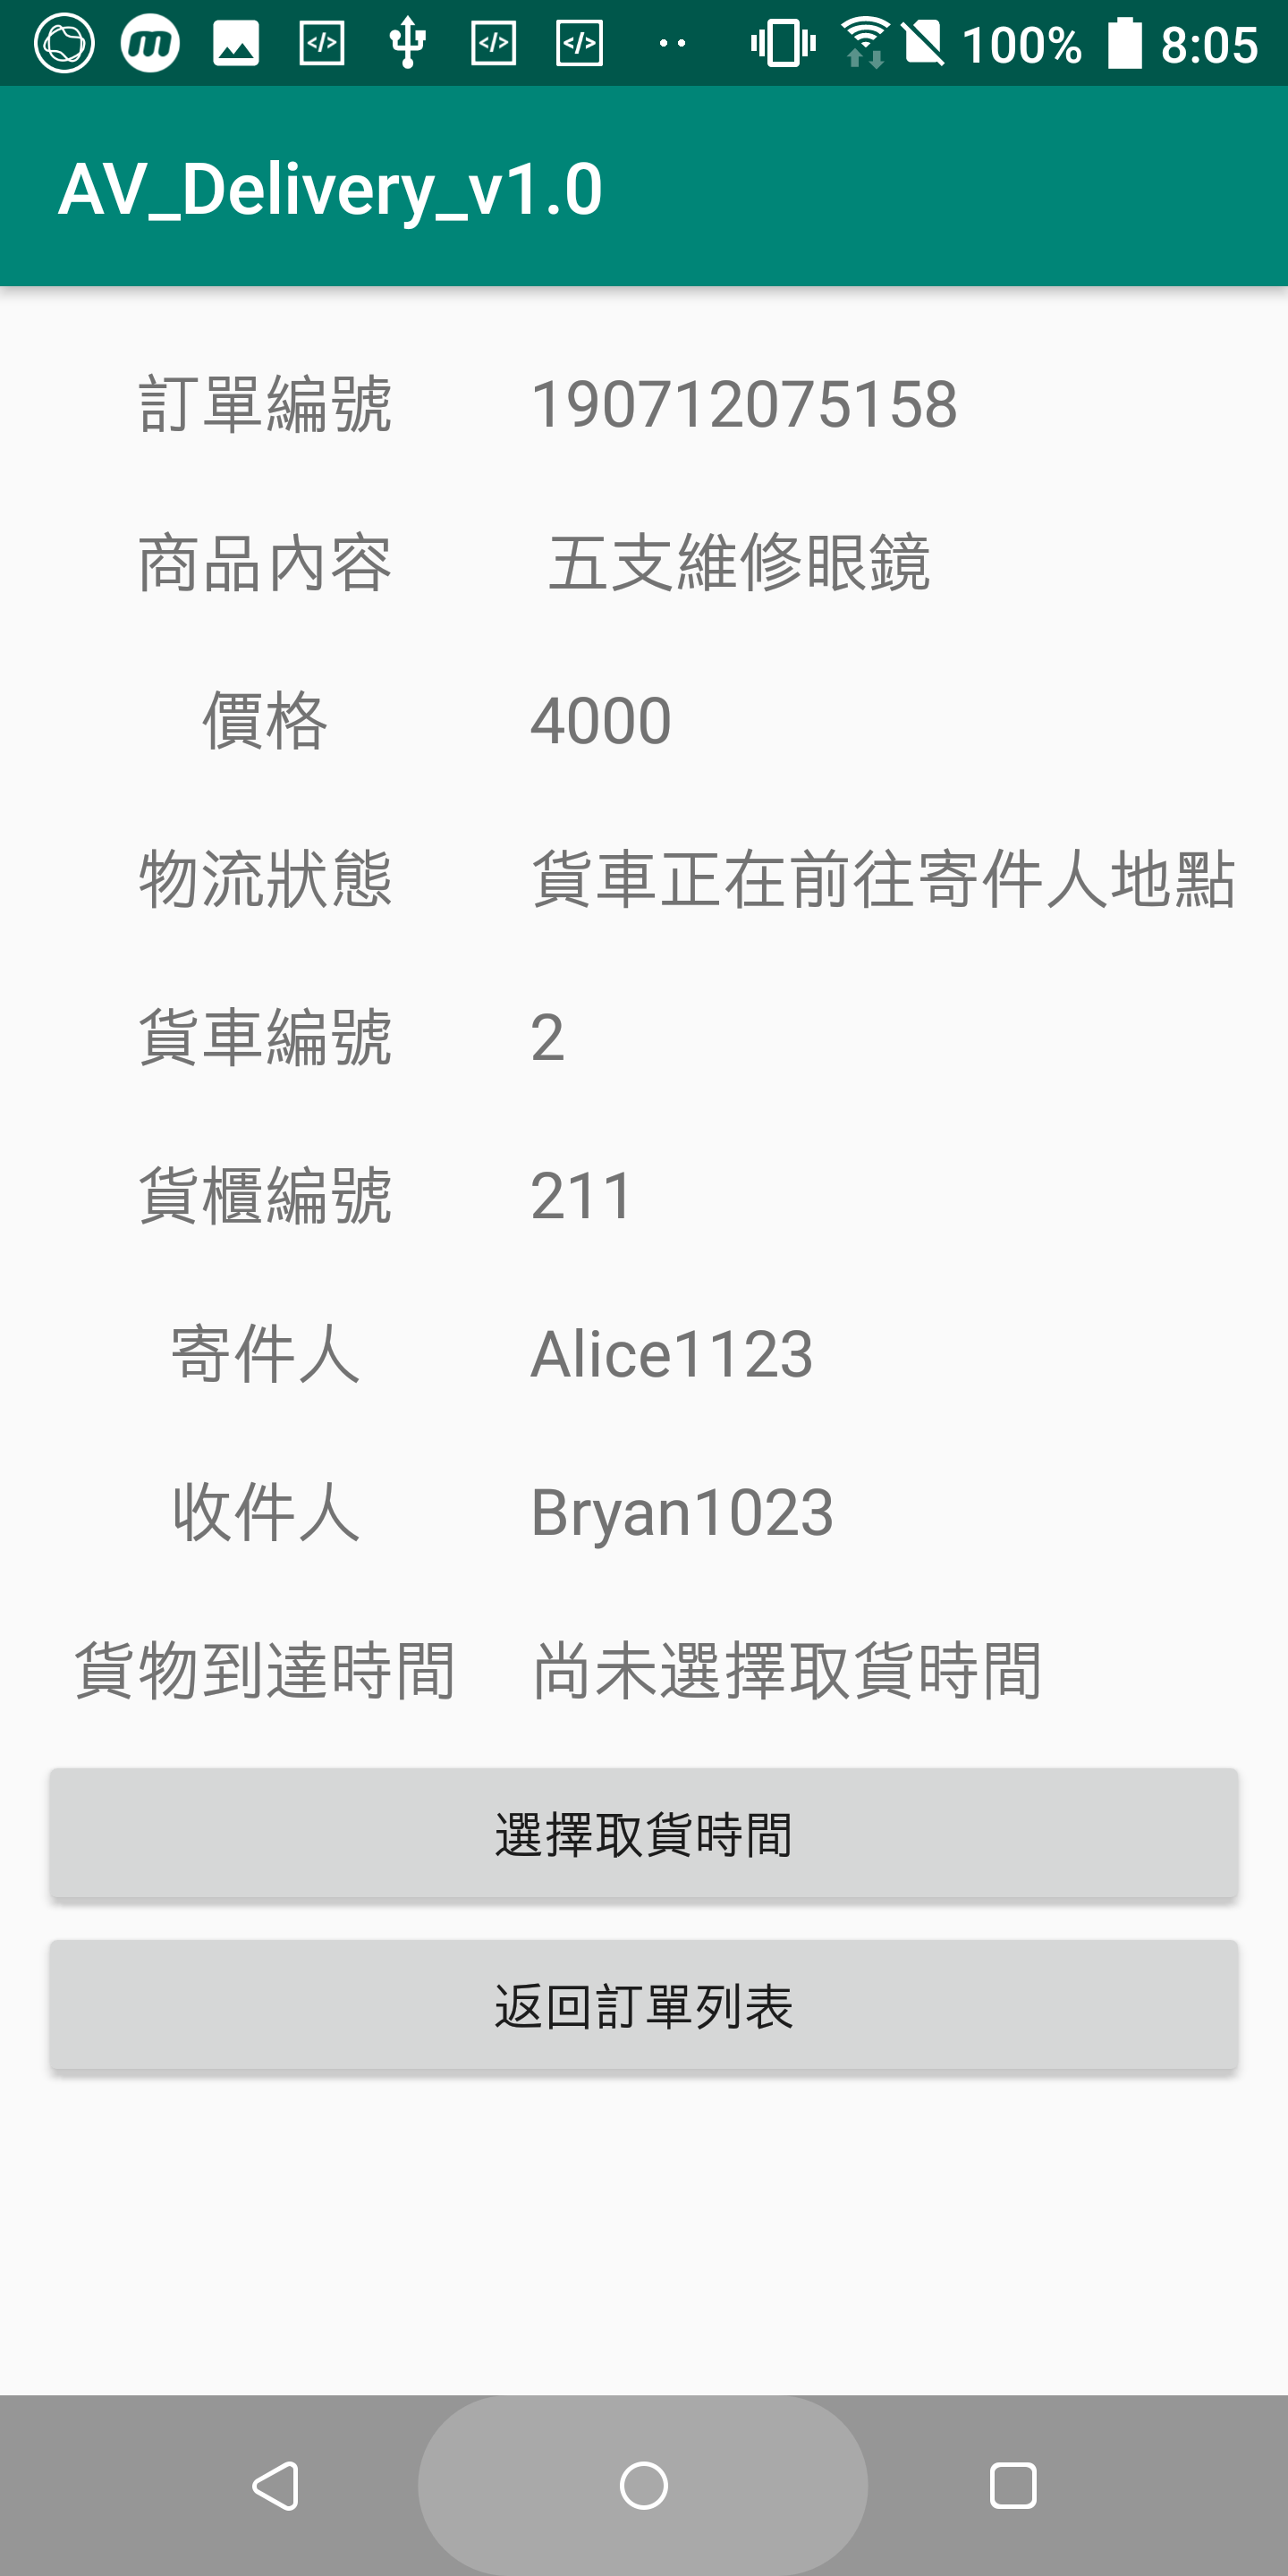
\includegraphics[scale=0.125]{./figures/F4-7-Details_package.PNG}
\caption{\large The details of the package.}
\vspace{0.5cm}
\label{Fig:details_of_package}
\end{figure} 


Then, the details of the appointed package would be displayed while the user clicks the order button, which is shown in Figure 4.7. 

If the user is a \textbf{receiver} in an order, he or she can choose the pick-up time of the cargo according to the \textbf{status of logistic activity}, which means the shipping situation of the cargo. Then, the \textbf{pick-up-time} page would pop up, which is same as the page in Figure 4.5. 

\begin{figure}[H]
\centering
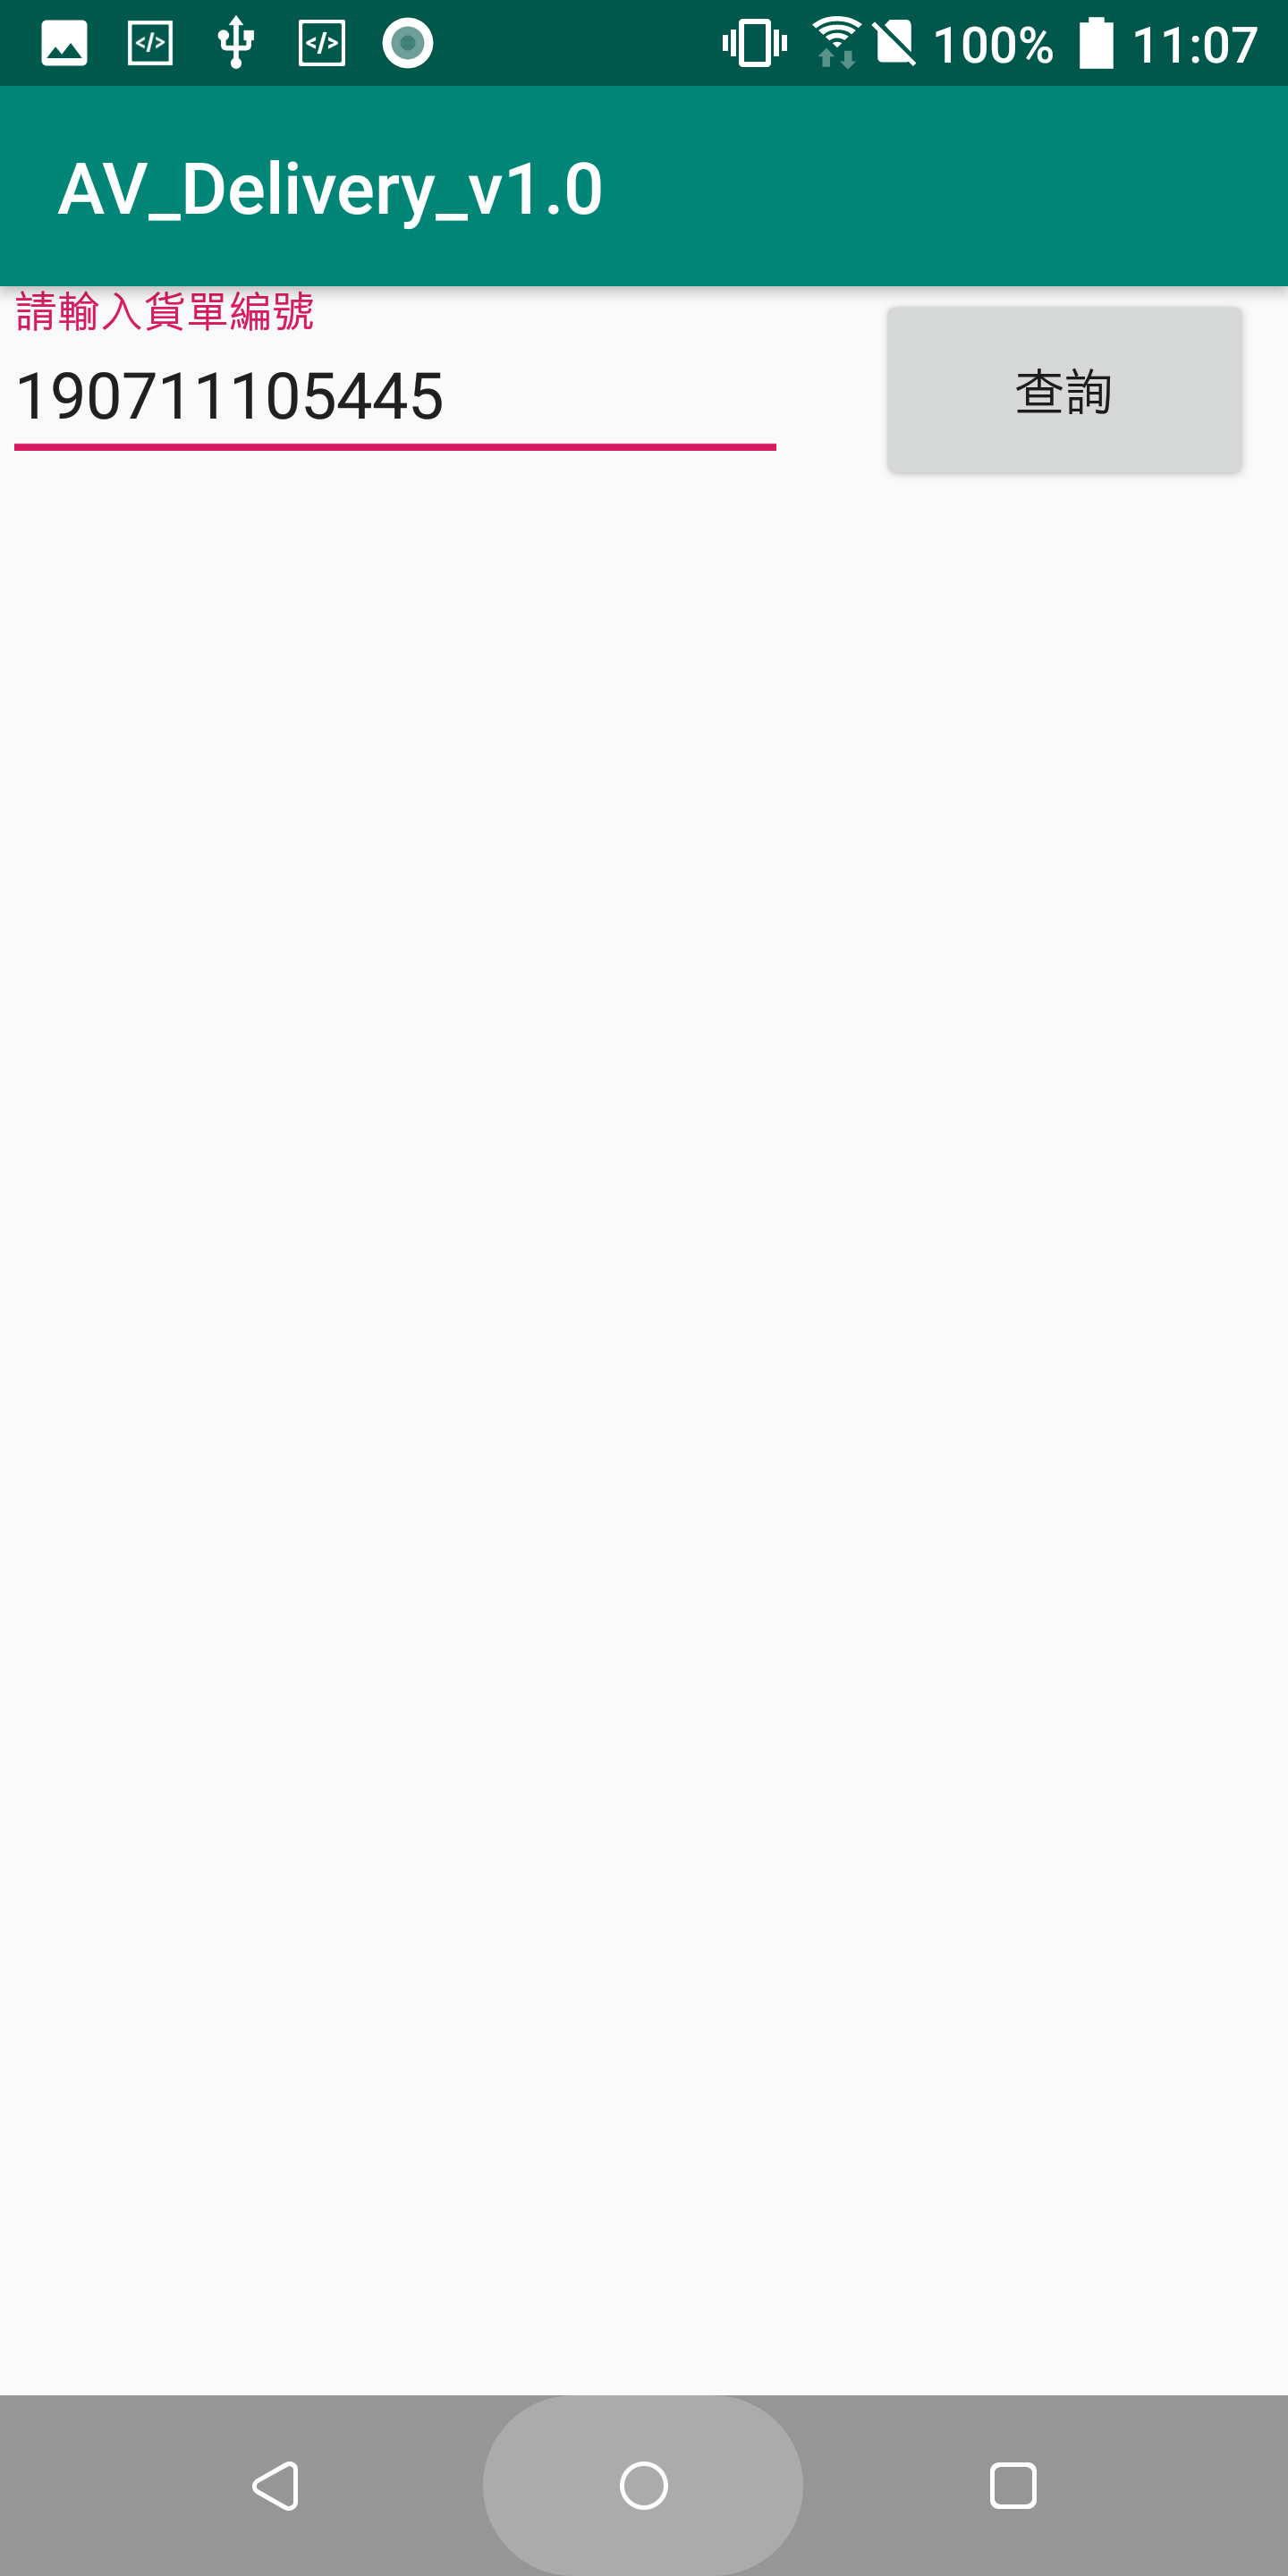
\includegraphics[scale=0.125]{./figures/F4-8-ExamineOrders.PNG}
\caption{\large Entering the order number to track the package.}
\vspace{0.5cm}
\label{Fig:ExamineOrders}
\end{figure} 


Besides, if a system administrator wants to examine the history orders without logging in. Thus, Figure 4.8 exhibits the searching page of the order, and the order can be looked up by entering the unique order number. 




\section{SUMO Server and Simulator}

\subsection{Simulation Environment Setup}

The simulation of the delivery process is implemented on SUMO, "Simulation of Urban Mobility", which is an open source, highly portable, microscopic and continuous traffic simulation package. The example of roads, vehicles, junctions and other road information are included in the package, and there is the graphical simulator certainly. TraCI is an interface that provides the access to SUMO simulator by using a TCP based client/server architecture. It was implemented in various programming language, such as Python, C++, Java, and so on. In this thesis, TraaS is employed to be the control interface of the simulator. It is a java library for working with TraCI, and it provides plenty of commands to manipulate the simulated objects. For instance, the developer can change the route of a vehicle by certain commands.

\begin{figure}[H]
\centering
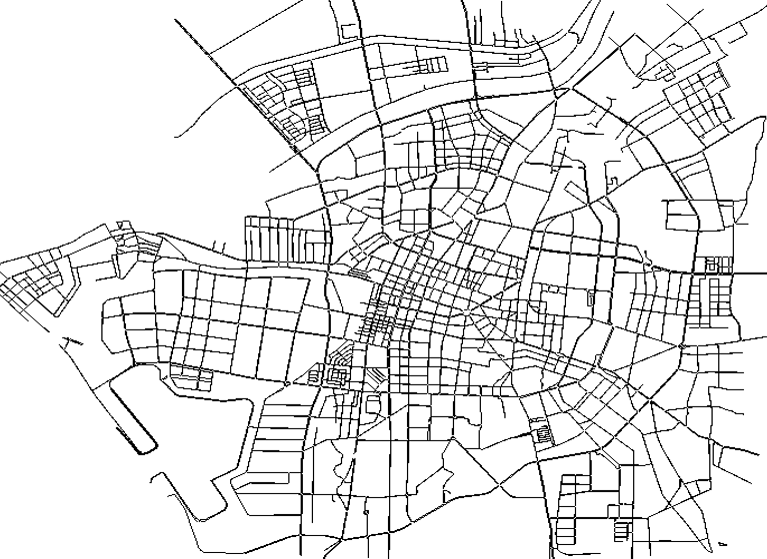
\includegraphics[width=1.0\textwidth]{./figures/F4-9-SUMOMap.PNG}
\caption{\large The service region on SUMO Map .}
\vspace{0.5cm}
\label{Fig:SUMOMap}
\end{figure}



The self-driving delivery system is designed to supply a small-scale package delivery service in cities. As illustrated in Figure 4.3, the road network environment of simulation is an approximate 50 $km^{2}$  area, which is a partial region of Tainan, a south city of Taiwan. The resource of the map data is gained from OpenStreetMap, which is a is a collaborative project to create a free editable map of the world. There are 25069 road segments and 6785 junctions in the simulation, and the traffic lights are deployed on the junctions using the real world data. In the beginning of the simulation, three trucks are generated on the roads randomly, and they drive along random routes until the end of the simulation. The maximum speed of trucks is set to 5 m/s according to the average speed estimated by Google Map. The delivery task can be assigned in any time.


\subsection{Build the Socket Server}
For purpose of communicating between the mobile application and the simulator, the thesis built a SUMO server to receive the data transferred from the mobile device which makes the simulator perform delivery task. The SUMO server is composed of a socket server and a main simulated program, which are both developed in Java language. This thesis copes with the socket server part and operations of database API.

When the simulation starts, the socket server will listen to the incoming connections from mobile applications. The socket server is programmed with a multi-client architecture, and the demand can be coped in a short period of time. Hence, the system can serve considerable users simultaneously. The user’s request will be stored in the request queue when the user connects to the socket server, and the data format of the request is represented by JSON (JavaScript Object Notation). The simulated program would check the queue in each simulation second. If there is any request, it will be forward to the dispatching mechanism. 

The order information would be uploaded to the database using JDBC if the dispatching execution is successful. JDBC (Java Database Connectivity) is an API for Java to access the database. The database and the SUMO server are built on the same computer because of the security concern. Then, the data can be transferred directly to the local side. 

\begin{figure}[H]
\centering
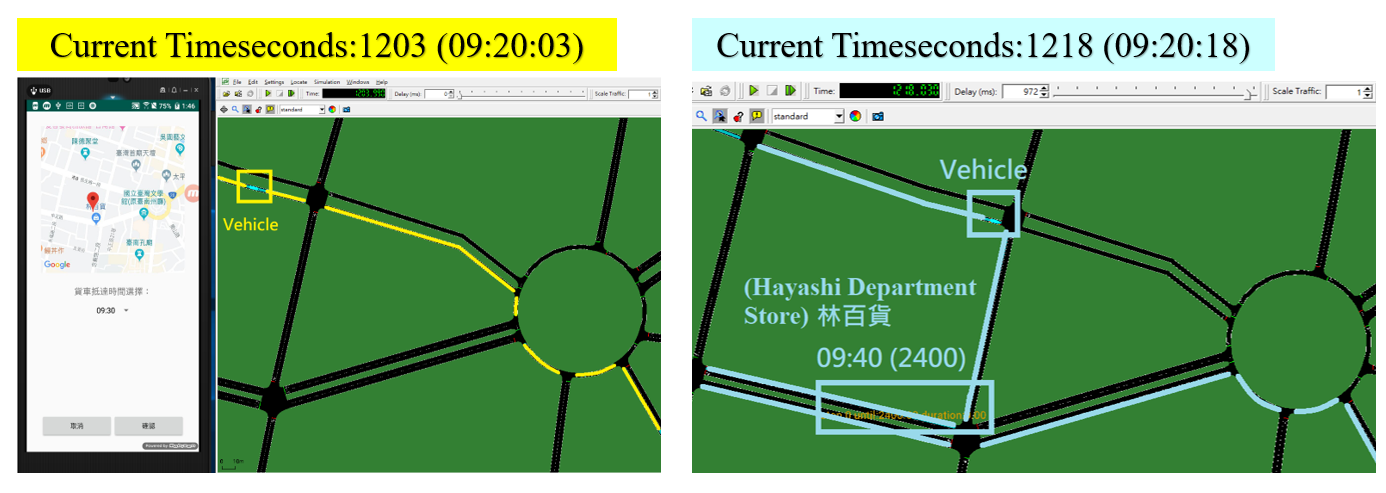
\includegraphics[width=1.0\textwidth]{./figures/F4-10-ChangeRoutes.PNG}
\caption{\large The changes of the route.}
\vspace{0.5cm}
\label{Fig:Change_of_route}
\end{figure}


Figure 4.10 shows the change of the routes after dealing with the order request. 
In the left side of this figure, the vehicle follows the yellow route. However, after the dispatching command is appointed to the truck, the truck will follow the new route, whose color is blue in the right side of the figure. 
Thus, the simulation process will display on the GUI of the simulator so that the system administrator can confirm the information of trucks and containers. 

\begin{figure}[H]
\centering
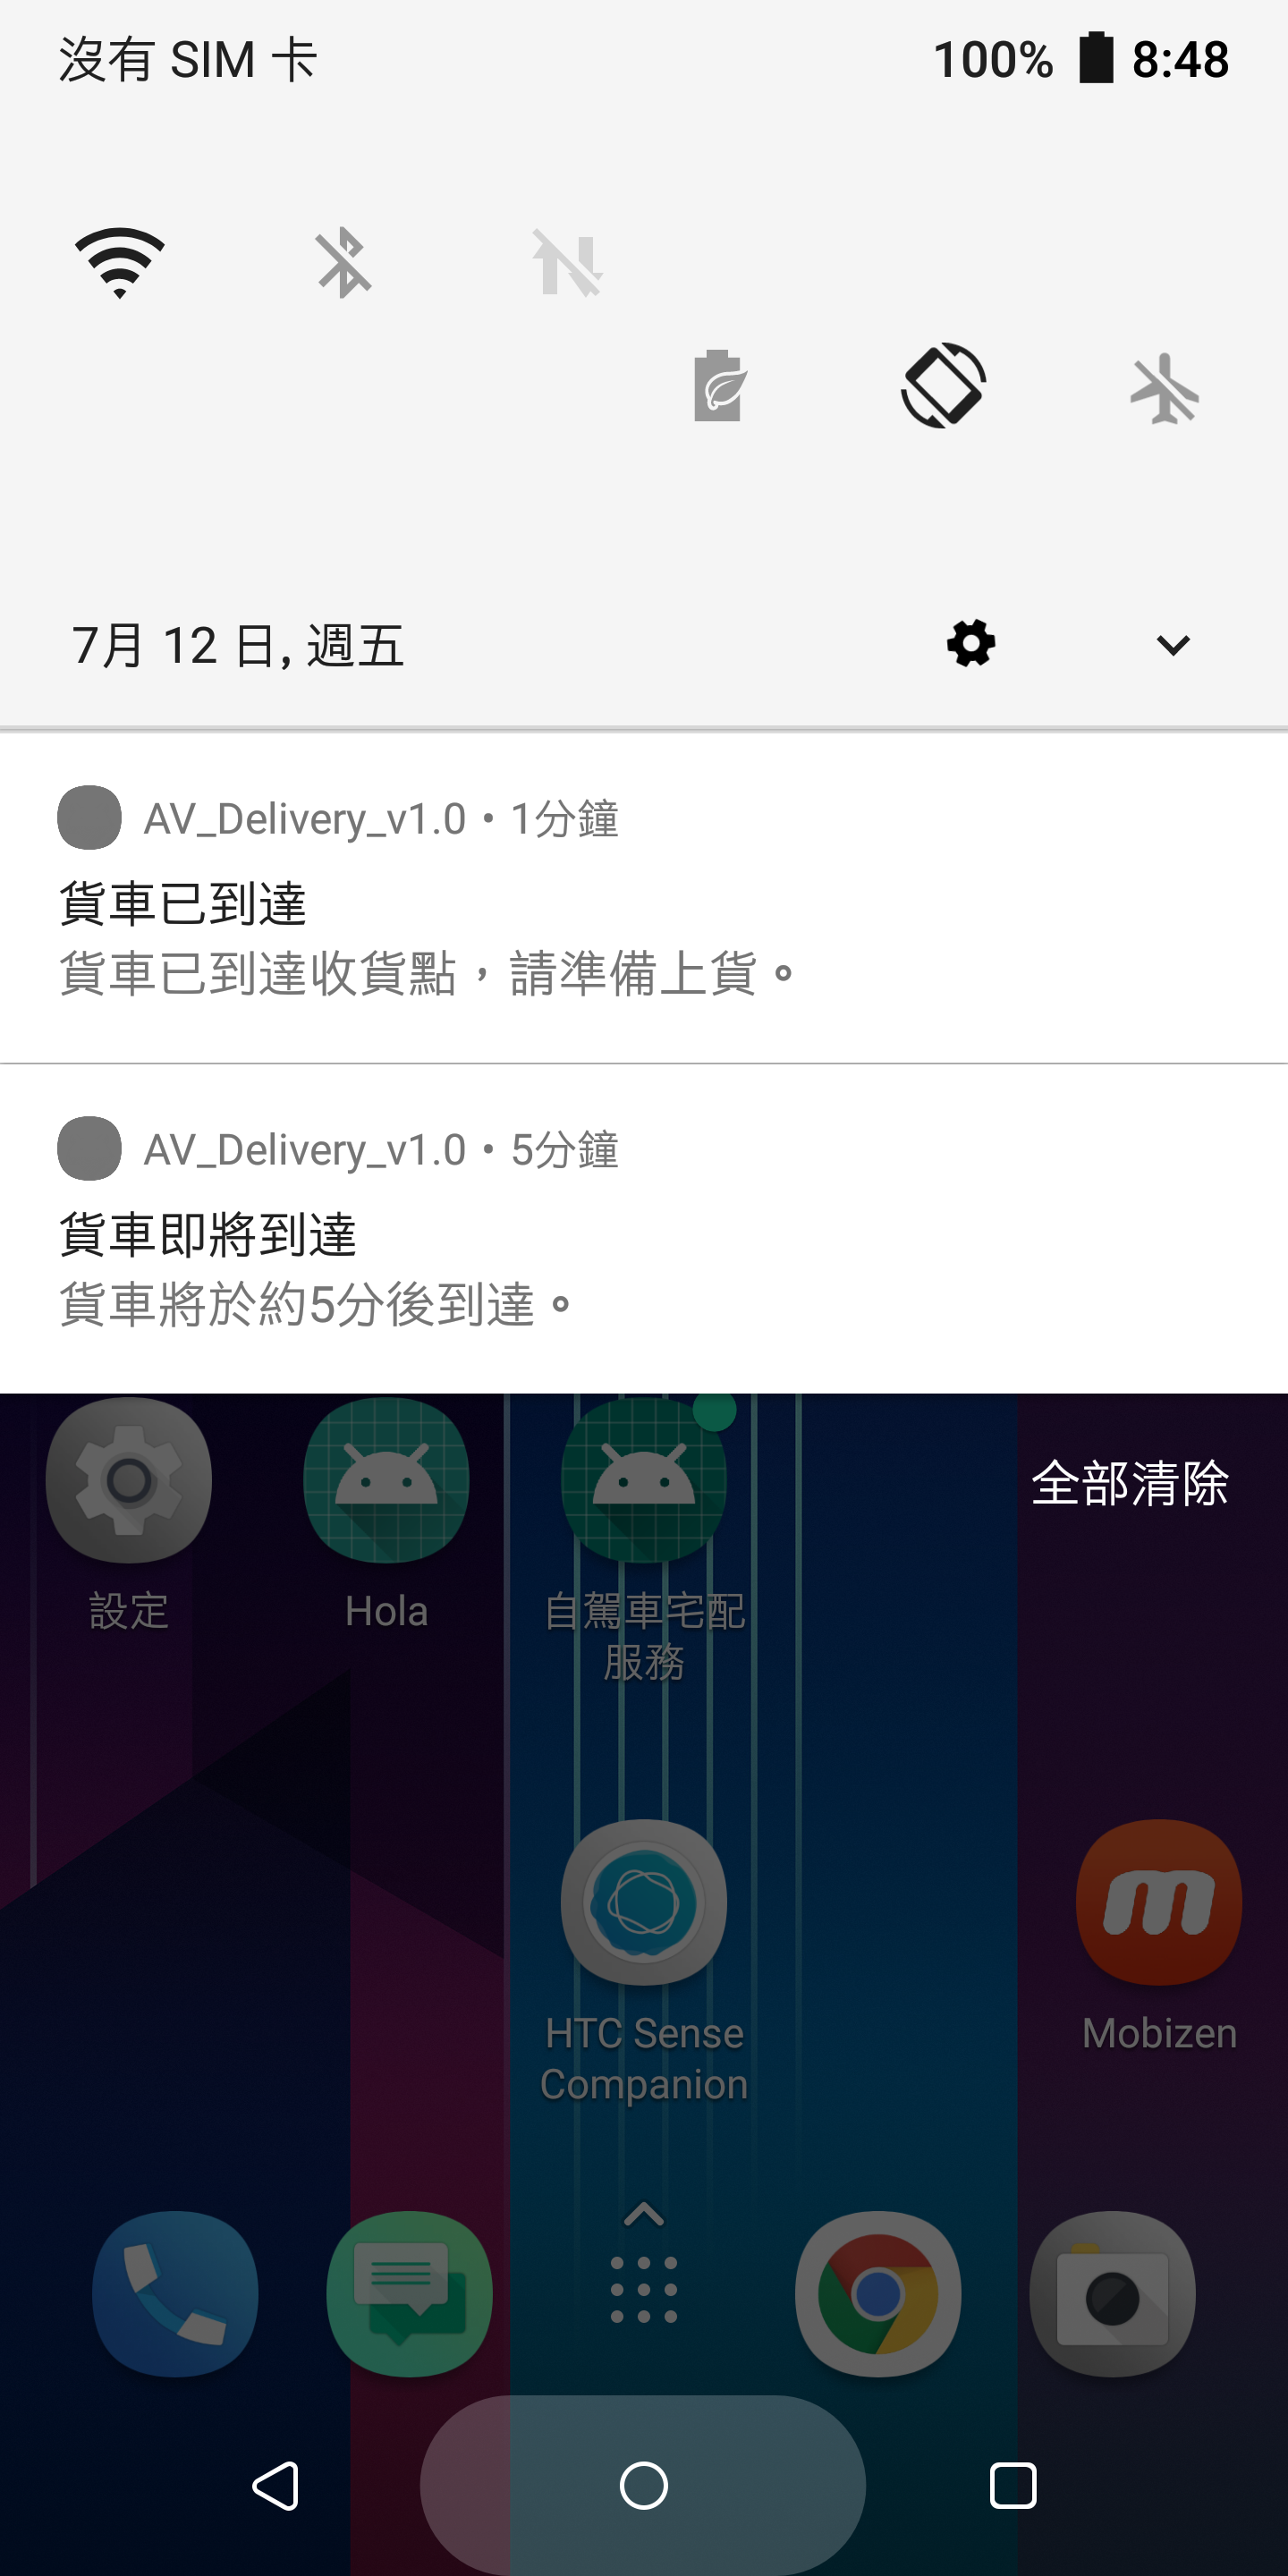
\includegraphics[scale=0.125]{./figures/F4-11-Notification.PNG}
\caption{\large The notification from FCM service.}
\vspace{0.5cm}
\label{Fig:Notification}
\end{figure} 


Figure 4.11 shows the mobile phone receives the notification from the FCM service. Moreover, the FCM service is also implemented in the SUMO server. 
When the truck is close to the destination, the system would notify the user of the coming message. Then, as the truck arrives to the destination, the system would inform the user of the arrival of the truck via FCM server.



\section{Back-end Sever}
To avoid the leakage of sensitive information of the database, users can not connect to the database directly. Thus, the system takes the back-end server as an interface to access to the database. The back-end server is a web server, which is built using Apache HTTP Server. The service which receives query requests from users, and the service is implemented with PHP program. 
The mobile applications connect to the back-end server by HttpUrlConnection. It is Android function which makes the application communicate with the web server by HTTP protocol. According to the HTTP URL, the web server would run the PHP program to execute the SQL commands of the database. The result returned from the database will be forwarded to the mobile application by the web server. 


\section{Database}
The database of the system is developed with MariaDB 10.1.32. MariaDB is a community-developed, commercially supported fork of the MySQL relational database management system. It inherits the advantages of MySQL. Hence, MariaDB supplies the JDBC driver, and the database API for PHP. This is highly useful for the development of our system. To deal with the administration of the database, phpmyadmin is employed in this thesis, it is a graphical, free and open source tool written in PHP. It allows the developer to manage the database with the use of a web browser. The records of orders can be exported for the subsequent data analysis.

The current goal of the system is to achieve the urban-wide delivery process. Therefore, the information of the administrative districts is stored in county table and township table of the database. There are three cities in county table currently, including Tainan City, Taichung City, and Taipei City. In the simulation of this thesis, only the map of Tainan City is constructed in the simulator, and the simulated districts involve East District, West Central District, North District, South District, Anping District and Yongkang District. The data are referenced from the Ministry of the Interior’s Open Data (MOI Open Data).








%----------- Simulation --------------%



%%%%%%%%%%%%%%%%%%%%%%%%%%%%%%%%%%%%%%%




\chapter{Conclusion and Future Work} \label{Chap:Conclusion}
%------------------------- Conclusion -------------------------%

\section{Conclusion}
In order to make the self-driving technology development companies have a platform to test and adjust the product before it is officially online, a system was designed and implemented to simulate the freight process of the self-driving delivery. This thesis handled the developing of a mobile application and the data transmission between apps and the simulation system. In terms of the mobile apps, an account system was accomplished to store user information, and the order functions were devised to send and display orders. For the purpose of performing the dispatching mechanism, SUMO server must be able to interact with mobile apps. Therefore, a socket server was built to receive and handle the data sent by apps. For similar reasons, FCM service was also be included in the system, and it can assist SUMO server in notifying users of mobile apps. As regards the database, a back-end server was built to supply the access interface of the database to the mobile apps. In contrast, SUMO server transfers data to the database directly because it is on the inner server side.


\section{Future Work}



\cite{Savelsbergh2016} Savelsbergh2016

\cite{Crainic2015}55

\cite{Habault2019}




} \end{thesis}

%------------------------- References -------------------------%
\singlespace {\large

\bibliography{Reference-Po}

}

\bibliographystyle{IEEEtran}



\doublespace

\begin{vita}
%------------------------- Vita -------------------------%
\Thesisspace \large{


}\end{vita}

\end{document}

